\documentclass[
  BCOR=10mm, % Binding correction ([default=0])
  DIV=12, % Number of divisions for the page spread construction ([default=9])
  twoside, % two sided ([default='oneside'])
  headsepline, % separate head-line from content optically (horizontal row) (KOMA-Doc, Ch.'Kopf- und Fusszeilen')
  listof=totoc, % include list of tables/figures to list of content
  bibliography=totoc, % include list of literature to list of content
  index=totoc, % include index to list of content
  abstract=true, % Put an coresponding header to the abstract ([default='abstractoff'])
  numbers=noenddot, % suppress ending dot in numberations (required? -> 'pointednumbers')
]{cs-thesis}

\hyphenation{
  Infini-Band
  Soft-ware
  Soft-ware-Stack
  Open-Fa-brics
}

\addbibresource{literature.bib}
\usepackage{minted}


%%%%%%%%%%%%%%%%%%%%
%%% THE DOCUMENT %%%
%%%%%%%%%%%%%%%%%%%%

\begin{document}

    %
% intro.tex
%

% start with non paging
% note: authorship itself has another empty
\pagestyle{empty}

% title (includes acknowledgment/dedication)
\maketitle

% authorship
\makeauthorship

% abstract
\makeabstract

% Zusammenfassung auf deutsch
% \cleardoubleemptypage
%\makezusammenfassung

% table of contents
\cleardoubleemptypage
\pagenumbering{roman}
\pagestyle{plain}
\tableofcontents
 % Title, abstract, ToC, etc. 
    
    % prepare main document
    \ofoot[\pagemark]{\pagemark} % show page numbering on chapter starts
    \nocite{*} % show all references in bibliography, no matter if used or not
    \cleardoublepage
    \pagenumbering{arabic}
    \pagestyle{chapterstyle}
    
    \acresetall % reset acronym counter
    %
% chapter1.tex
%

\chapter{Einführung}
\label{cha:introduction}

In modernen Rechnernetzen und Rechenzentren hat sich der Bereich der Lastverteilung zu einem der wichtigsten Teilbereiche entwickelt. Hintergrund ist, dass mit steigender Anzahl von Internetnutzenden die entsprechenden Hardwareressourcen nicht nur zur Verfügung gestellt werden müssen, sondern vielmehr eben auch die effiziente Nutzung von Interesse geworden ist.\cite{tanenbaum2007modern} Dabei gibt es verschiedene Ansätze und auch verschiedene Punkte, an denen Maßnahmen getroffen werden können, um eine breite Nutzung zu realisieren. Auch vor dem Hintergrund der globalen Erwärmung ist es sinnvoll, die Hardwarenutzung zu optimieren, da somit Energie eingespart und fossile Mittel geschont werden können. \cite{barroso2007case} \newline \newline
So wurden bereits relativ früh skalierbare Systeme entwickelt. Ein klassisches Beispiel ist hierbei der Einsatz von mehreren Prozessoren in Webservern der frühen 90er Jahre. Während dieser Zeit gab es technologische Vorstöße im Bereich des Internets für zivile Endanwender, wodurch dementsprechend die Nachfrage nach bereitstellender Rechentechnik stieg. Somit wurde indirekt die Zeit der Mehrkern-Prozessoren eingeläutet, obwohl diese erst Jahre später entwickelt wurden. Einen sehr ähnlichen Ansatz verfolgen die Entwickelnden moderner Lastverteiler. Dabei wird Wert auf eine horizontale Skalierung gesetzt. Es werden Ressourcen auf horizontaler Ebene nebeneinander gesetzt, um den Gesamtdurchsatz des Systems zu erhöhen. Der dem entgegenstehenden Ansatz wäre die vertikale Lastverteilung, bei der im Wesentlichen die Punktleistung eines Rechners erhöht wird. Auch die horizontale Skalierung findet breite Anwendung. Am wichtigsten hierbei ist das Hochfrequenz-Trading am Aktienmarkt, sowie High-Performance-Computing im Allgemeinen. \newline \newline Allerdings hat sich mit der zeitlichen Weiterentwicklung nicht nur das Interesse an Parallelisierbarkeit gesteigert, sondern ebenfalls ein Interesse an Hardwarearchitekturen, die im Gegensatz zum klassischen Prozessor nicht nur einen allgemeinen Zweck erfüllen, sondern für spezifische Anwendungsbereiche entwickelt werden. Dabei kann durch das an die Anwendung angepasste architektonische Layout dermaßen optimiert werden, dass es nicht nur zur Leistungssteigerung selbst kommt, sondern eben auch zu einer deutlich besseren Energieeffizienz. Zudem haben die letzten Vorstöße im Bereich des maschinellen Lernens dazu geführt, dass eine Menge der traditionellen Rechenzentrumsarchitekturen zwar für die modernen GPU-Cluster funktionieren, es aber eine Menge an Potenzial und Optimierungsspielraum gibt. \cite{jouppi2017datacenter} \newline \newline Diese Arbeit behandelt eben genau eine dieser modernen Technologien, die zwar mit einer Idee für einen Anwendungszweck ins Leben gerufen wurde, aber die tatsächliche Anwendung noch immer hinterherhinkt.
    
    \acresetall % reset acronym counter
    %
% chapter2.tex
%

\chapter{Smart NICs - ein Überblick}
\label{cha:background}

\section{Begriffserklärung}
Der Begriff \textbf{Smart Network Interface Card} (Smart NIC) ist wie allzu oft in der Computerwissenschaft mit einer Menge von Definitionen versehen. Grundsätzlich beschreibt eine Smart NIC eine Hardwareeinheit, die sich mit der Netzwerkfähigkeit eines Rechners beschäftigt. Dabei unterscheidet sie sich von den klassischen Netzwerkkarten in der Hinsicht, dass wir als Anwender beziehungsweise Entwickler Anwendungen schreiben können, die das Verhalten der Karte beeinflussen. Dabei ist nicht fest definiert, welche Funktionen gebaut werden oder überhaupt in welchem Umfang Programmierung stattfinden kann. Nicht zuletzt ist das immerwährende Aufkommen des Begriffs Smart* dafür verantwortlich, dass sicherlich auch aus Marketinggründen ein etwaiger Name gewählt wurde. Allgemein ist eine Smart NIC eine Netzwerkkarte, die es erlaubt, Anwendungen zu erstellen, die ihr eigenes Verhalten derart verändern kann, dass Funktionen, die sonst innerhalb eines Netzwerkstapels übernommen werden würden, nun auf der Netzwerkkarte selbst ausgeführt werden können. \cite{smartnicsComproSurvey}

\section{Aufbau und Funktionsweise}
Smart NICs verwenden unterschiedliche Hardwarearchitekturen, um eine Hardwarebeschleunigung zu realisieren. Allgemein gab es sogar in den 90er- und frühen 2000er-Jahren Smart NICs, die lediglich oder größtenteils klassische Prozessorarchitekturen wie RISC oder x86 verwendeten. Mit Anbruch des neuen Jahrtausends jedoch zogen immer mehr FPGA- und ASIC-basierte Architekturen in die Rechenzentren ein. \cite{towardsSmartNICCluster}
\begin{figure}
    \centering
    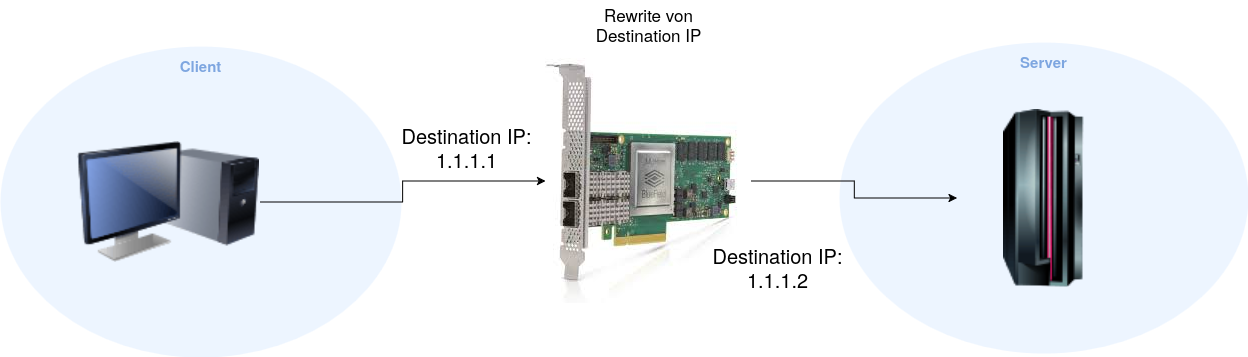
\includegraphics[width=1\linewidth]{images/GrundaufbauSmartNIC.drawio.png}
    \caption{Einfaches ändern einer IP Adresse im Paket}
    \label{fig:enter-label}
\end{figure}
Das steigende Interesse an der SmartNIC Architektur ist nicht zuletzt durch den abflachenden Leistungsgewinn durch Generationsfortschritte in der Prozessorindustrie befeuert worden. Mittlerweile gilt das Moorsche Gesetz als beendet und ein Großteil der Computerkommunikation heutzutage ist ohnehin Netzwerkverkehr. \cite{endofmoore} Meistens werden dazu TCP- und UDP-Pakete verwendet. Werden diese Pakete auf Prozessoren verarbeitet, sind die entsprechenden Kosten nicht nur hardware-, sondern auch energieseitig sehr hoch. Zuletzt hat nun auch der Aufschwung der modernen Softwarearchitekturen für einen explosionsartigen Anstieg in Netzwerkverkehr gesorgt. Wurden vor 20 Jahren Anwendungen noch so entwickelt, dass möglichst wenig Kommunikation über ein Netzwerk läuft, wird in heutigen Systemen stark und immer mehr auf eine Microservice-basierte Architektur gesetzt. \cite{microservices} Dabei wird eine komplexe Applikation in verschiedene Bereiche unterteilt, die daraufhin mittels HTTP angebundenen Interfaces miteinander kommunizieren. Grund dafür ist die Idee der vereinfachten Wartbarkeit von kleinteiligen Applikationen.
Zu Beginn der Entwicklung besagter Hardware war zunächst grundsätzlich die Idee, die programmierbare Funktionalität auf dem Switch, also dem Anbindungspunkt des Rechenzentrums, umzusetzen. Allerdings steigt mit der Anzahl der Knoten im Teil hinter dem Switch auch die benötigte Rechenkapazität des Switches. \cite{smartswitches} Daher hat sich ein eher dezentraler Ansatz entwickelt, bei dem in dem Server selbst eine Karte integriert ist, auf der sich ein zusätzlicher Rechner befindet. Dabei ist die Verbindung zugunsten der größten Kompatibilität meist mittels PCI Express umgesetzt. In der Abbildung 2.1 ist ein grundsätzliches Diagramm eines hier erstmal abstrahierten Datenpakets dargestellt. Der Client schickt ein Paket mit einer bestimmten Ziel-IP-Adresse los und zu einem gewissen Zeitpunkt erreicht das Paket die Smart NIC. Diese wendet daraufhin eine Aktion an. In diesem Fall wird die Ziel-IP-Adresse geändert und zurück in das Netzwerk geleitet. Dadurch bekommt nun ein anderer Server das Paket. Hierbei ist interessant, dass die Umleitung dem Client verborgen bleibt. Im Prinzip handelt es sich also bei dem gezeigten Beispiel um einen primitiven L3-Proxy.
\subsection{Hardwareaufbau}
SmartNICs sind in aller Regel im Grunde völlig eigenständige Systeme, mit einer Prozessoreinheit, Arbeitsspeicher und teilweise sogar eigenständiger Netzwerkein- und -ausgabe über einen separaten Hardwareport. Die Idee dabei ist es, ein System zu schaffen, auf dem eigenständig Applikationen ausgeführt werden können, aber auch Dienste wie Docker oder Kubernetes angewendet werden können. So wird auch die Verbindung zur Entwicklung über etwaige Dienste wie SSH hergestellt. Allerdings bieten auch einige Hersteller eigenständige Lösungen an, welche in aller Regel mittels \textbf{\textit{Application Programming Interfaces}} kurz APIs zur Verfügung gestellt werden. Hauptgrund ist allerdings wie so oft in solch hochkritischen Systemen Sicherheitsbedenken. Eine vollständig getrennte Einheit unterstützt in diesem Sinne das Konzept der Zero-Trust-Paradigmen. Dabei ist die Grundannahme, dass alle Kommunikationspartner sowie alle Beteiligten in einem System nicht zu vertrauen ist. Eine SmartNIC kann somit völlig autark in einem Netzwerk fungieren, ohne dass das Hostsystem selbst den Aufbau des Netzwerks oder dessen Funktionsweise kennt. \cite{whatyouneedtoknowaboutsnics} Die besonders im Kontext der Netzwerkverarbeitung relevanten Hardwareeinheiten werden mittels fest verarbeiteter Hardwareinterfaces angesprochen. Dabei werden meist die vorliegenden PCI Lanes als Hochgeschwindigkeitsverbindung genutzt. Und genau hier wird auch einer der größten Unterscheidungspunkte zwischen der klassischen Netzwerkpaket verarbeitenden Hardware und den SmartNICs deutlich. Die meisten anderen Netzwerkadapter verwenden klassische Mikrocontroller, um eine Konfigurierbarkeit zu gewährleisten. Die Kommunikation zwischen den Mikrocontrollern und den tatsächlichen Hardwarebeschleunigern findet daraufhin meist mittels serieller Schnittstellen statt. Dabei ist natürlich das Hauptunterscheidungsmerkmal unter anderem der Prozessortakt. Klassische SmartNIC \textbf{\textit{Systems on a Chip}} kurz SoC verwenden Prozessoren mit mehreren Kernen, die in einem ähnlichen Bereich getaktet sind wie etablierte Server- oder Desktopchips. Dabei ist die Leistung vor allem relevant, da auch klassische Berechnung auf den Kernen ausgeführt werden sollen. Bei den kleineren, schwächeren Mikrocontroller-Prozessoren liegen die Taktraten größtenteils klar unter 1 GHz. Diese werden allerdings auch eben nur für Konfiguration und Management verwendet und übernehmen keine direkte Aufgabe, die an der Paketverwaltung beteiligt ist. Zusammenfassend lässt sich also eine grobe Unterteilung vornehmen, bei der die SoC Varianten von SmartNICs klar von denen unterscheiden die diskrete Hardwareeinheiten für den jeweiligen Verwendungszweck besitzen.
\subsection{Path Switching}
Über die letzten Jahre haben sich unter diversen anderen architektonischen Ansätzen zwei etabliert, welche für den Kontext dieser Arbeit von besonderer Bedeutung sind. Dabei wird die hauptsächliche Unterscheidung dadurch getroffen, dass unterschieden wird, wo genau die Switching-Funktionalität stattfindet. Es wird grundsätzlich zwischen On-Path-Switching und Off-Path-Switching unterschieden (siehe Abbildung 2.2).
\subsubsection{On-path SmartNICs}
Bei einer On-Path SmartNIC verhält sich die Netzwerkkarte sehr nahe an der Funktionsweise, wie man sie von einer traditionellen Netzwerkkarte erwarten würde. Pakete, die über das Kabel an die Hardware herantreten, werden zunächst von dem entsprechenden Stack der Karte verarbeitet und laufen gezwungenermaßen nicht nur über den Traffic-Manager, sondern insbesondere auch über die Kerne der SmartNIC. \cite{onoffpath} Das heißt zwar, dass ein nicht unerheblicher Overhead bei der Verarbeitung des Datenverkehrs im Kernel des Betriebssystems der Netzwerkkarte entsteht, ermöglicht es aber eben auch, Modifikationen an besagten Paketen vorzunehmen. Dabei steht aber vor allem auch die vereinfachte Entwicklung solcher Netzwerkkarten im Vordergrund. Sollte es sich wiederum um eine On-path SmartNIC handeln bei der Paket direkt über den Kernel des Hostrechners verarbeitet werden stellt sich hierbei das Problem da, dass es so zu einer Überlastung der Anbindung zwischen SmartNIC und Host kommen kann. Außerdem liegt in solch einem Fall dann ein großteil der Rechenlast wieder beim Host, womit die eigentliche Funktionalität der SmartNIC stark abnimmt. 
\subsubsection{Off-path SmartNICs}
Bei Off-Path SmartNICs handelt es sich hingegen um Geräte, bei denen eine klarere Trennung der Hardwareeinheiten vernommen wird. Eben diese Trennung ermöglicht es, eine Spezialisierung vorzunehmen, mit der für bestimmte Anwendungszwecke besondere Hardwarebeschleuniger verbaut werden können.  Diese Architektur erlaubt es, einen wesentlich größeren Anwendungsbereich abzudecken, da dadurch eine große Flexibilität für die Verarbeitung von Datenpaketen gewährleistet wird. Wenn ein Paket eintrifft, muss es nicht von einem Prozessorkern der Netzwerkkarte beachtet werden, sondern kann von der speziellen Hardwareeinheit verarbeitet werden. \cite{onoffpath} Dabei werden in aller Regel \textbf{\textit{Application Specific Integrated Circuits}} kurz ASICs verwendet. Die Konfiguration dieser ASICs erfolgt dann meistens mittels Software die auf dem Prozessor der Netzwerkkarte. Allerdings gibt es dort auch Unterscheidungen ob die Anwendung zur Konfiguration auf dem Hostsystem, also dem Rechner in dem die SmartNIC eingebaut ist oder der Karte selbst ausgeführt werden soll. Off-path SmartNICs verbessern somit die gesamt Architektur indem sie die Allgemeinen Kerne des Prozessors klar vom kritischen Pfad der Netzwerkpakete trennen und es so verhindern, dass die logische Last, welche mit einer Anwendung einhergehen kann, sich in keinster Weise auf den tatsächlichen Durchsatz der Netzwerkkarte auswirken können.
\begin{figure}
    \centering
    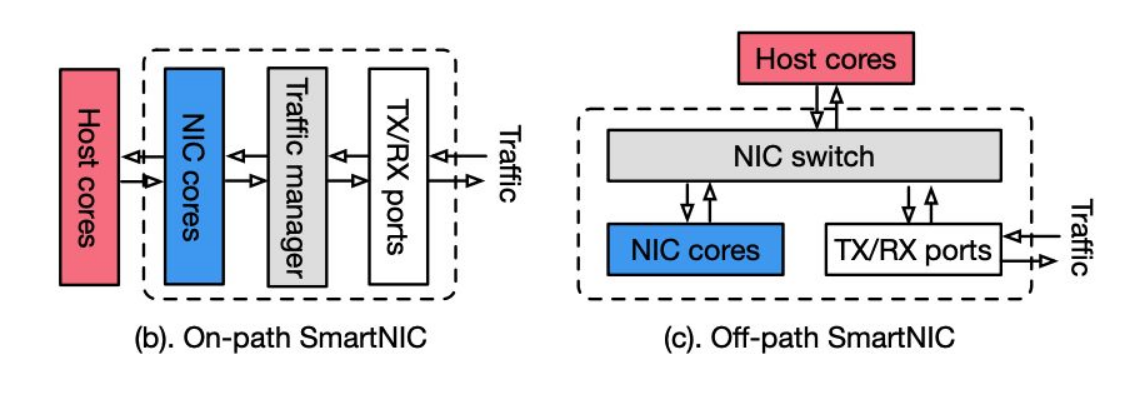
\includegraphics[width=0.9\linewidth]{images/Screenshot 2025-03-16 at 10-41-14 Netdev 0x14 -- Taking Control of your SmartNIC v1.pdf.png}
    \caption{On-Path vs. Off-Path-Switching \cite{onoffpathpic}}
    \label{fig:enter-label}
\end{figure}
\begin{figure}
    \centering
    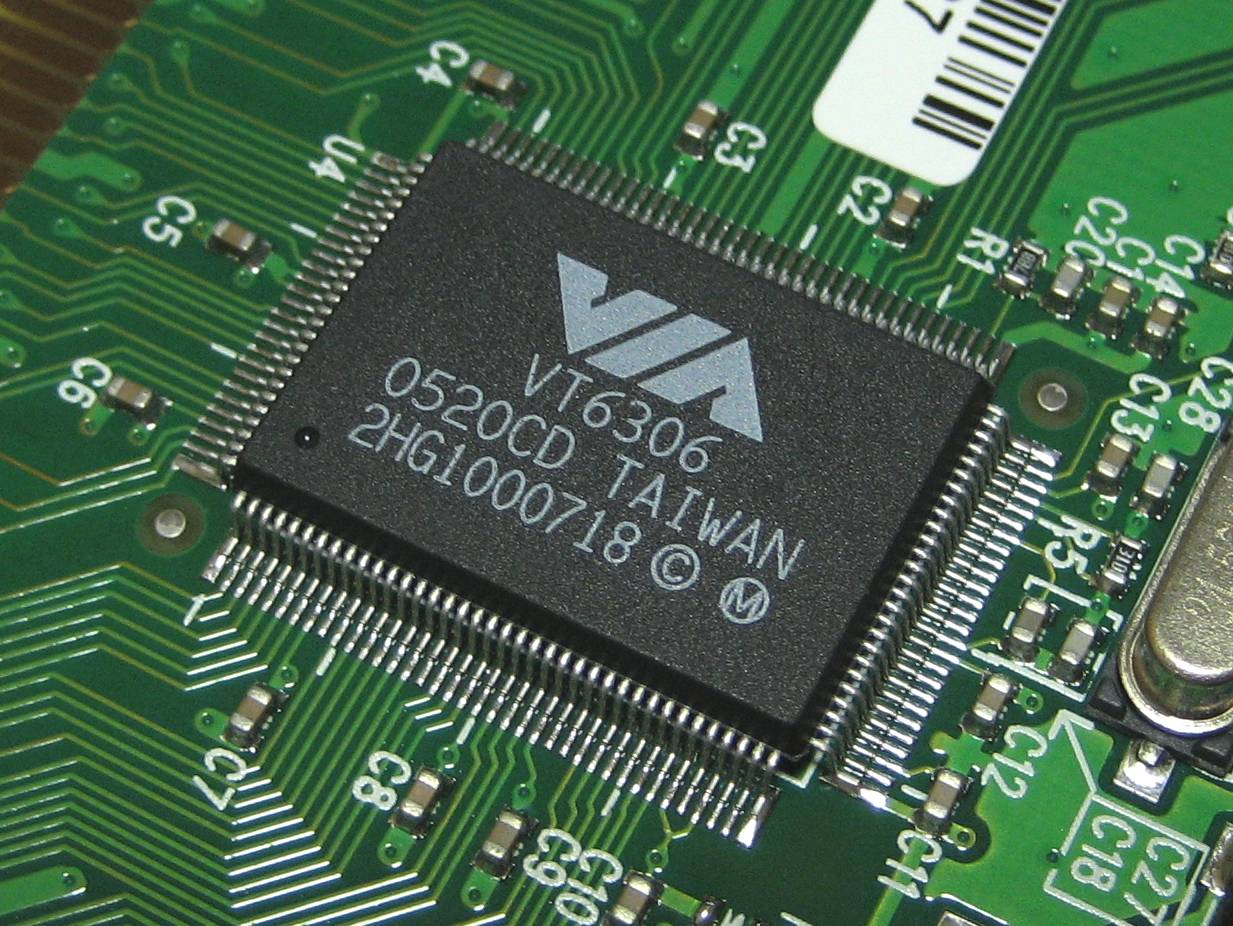
\includegraphics[width=0.5\linewidth]{images/Buffalo_IFC-ILP4_VIA_VT6306.jpg}
    \caption{Firewire ASIC - VIA CT6306 \cite{firewireasic}}
    \label{fig:enter-label}
\end{figure}
\subsection{Application Specific Integrated Circuits}
\begin{figure}
    \centering
    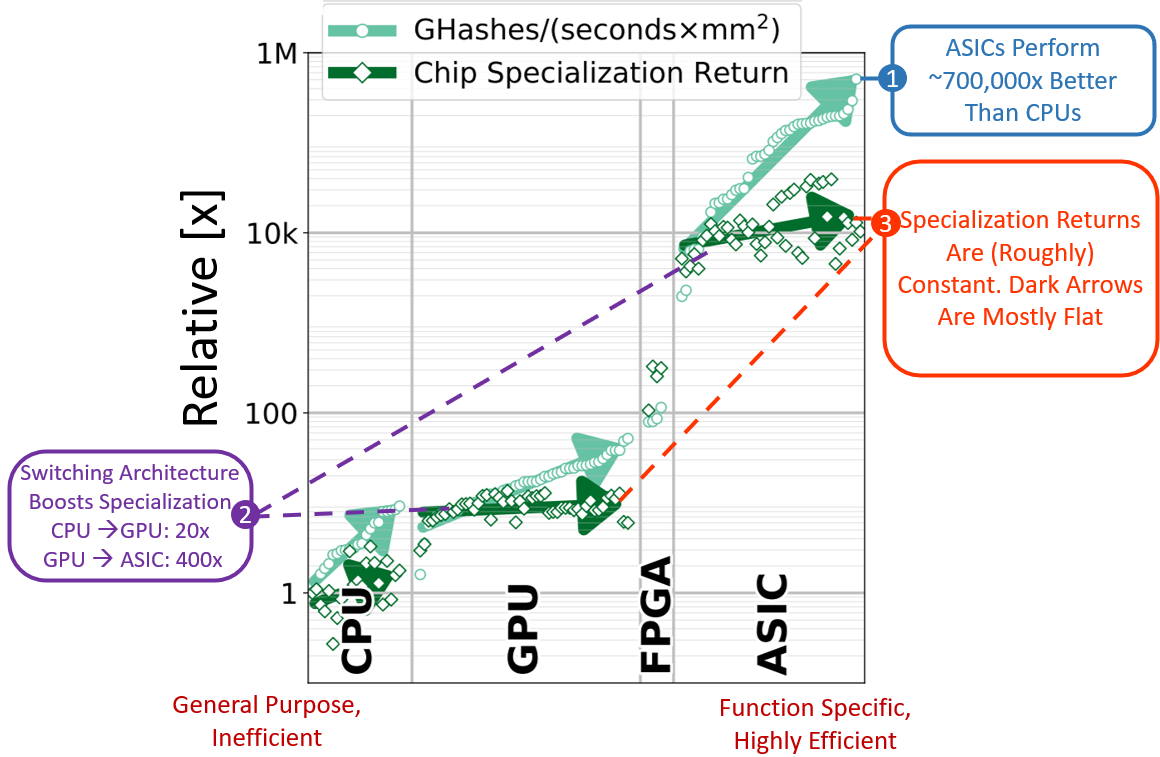
\includegraphics[width=0.7\linewidth]{images/aisic.png}
    \caption{Hardware Architekturen beim Bitcoin Mininig \cite{bitcoin}}
    \label{fig:enter-label}
\end{figure}
\textbf{Application Specific Integrated Circuits} (ASICs) sind Hardwareeinheiten, die ein sehr großes Anwendungsgebiet entwickelt haben. So werden sie nicht nur in Netzwerkbeschleunigern verwendet, sondern werden immer dann verwendet, wenn der Zweck der Hardware sich gut beschreiben lässt und somit keine große Varianz an Aufgaben von der entsprechenden Einheit übernommen werden muss. So wird es nämlich den entsprechenden Ingenieuren erlaubt, statt eines allgemeinen Rechners eine hochspezialisierte Einheit zu entwickeln, bei der die Merkmale einer klassischen Prozessorrecheneinheit vernachlässigt werden können. Dadurch ist eine wesentliche Effizienzsteigerung möglich, die es erlaubt, mit wesentlich weniger Energie die gleiche Leistung zu erzielen, wie es sonst eine vergleichbare Recheneinheit bewerkstelligen würde\cite{asic}. Für rechenintensive Systeme hingegen lässt sich eben letzterer Nutzen, da somit der allgemeine Durchsatz angehoben werden kann und somit Systeme realisierbar sind, die mit der Anwendung klassischer Rechenwerke erheblich mehr Aufwand bedeuten würden. Zudem erzeugen solche Systeme deutlich mehr Abwärme und würden die Entwicklung somit auch vor ein thermodynamisches Problem stellen. Zuletzt sei noch erwähnt, dass der Überbegriff ASIC nur sehr allgemein ist und ähnlich wie bei Prozessoren noch keine Auskunft über die genaue Implementierung gibt. Es gibt viele Architekturen, die für ASICs zur Anwendung kommen, da eben auch die Gebiete weitreichend sind und sich sehr divers unterscheiden. In Abbildung 2.3 ist ein ASIC zu sehen, der die Kommunikation zwischen einem Prozessor und einem sogenannten FireWire-Anschluss eines Endgerätes realisiert. Es muss festgelegt sein, welcher Standard von Geräten mit besagtem Anschluss erwartet wird, um den Prozessor des Hostgerätes mittels eines ASICs zu entlasten.
\newline

Der Zeitgeist in der Computerwissenschaft färbte letztlich außerdem das immens steigende Interesse an Machine Learning ab. Proportional dazu stieg das Interesse an effizienterer Hardware an, da etwaige Lernprozesse extrem energie- und somit kostenaufwendig sind. Es zeigt sich aktuell ein gesteigertes Interesse daran, ASICs zu fertigen, die effiziente hochdimensionale Vektoroperationen umsetzen. Dazu gibt es bereits mehrere Ansätze, mit denen beispielsweise LLM auf einer ASIC-Architektur ausgeführt werden können (siehe Abbildung 2.5). Machine Learning bietet großes Potenzial, Energie mittels ASICs zu sparen, da bisher GPUs und CPUs zum Einsatz kamen, die beide große Energiekosten mit sich bringen. So erlauben ASICs eine extreme Effizienz im Hinblick auf Leistung/Energiekosten (siehe Abbildung 2.4).

Abbildung 2.4 zeigt deutlich, wenn auch etwas vage, dass ASICs, sowie alle anderen Architekturen in sich selbst nur leichtes Leistungswachstum aufzeigen. Verwenden wir allerdings unterschiedliche Architekturen, so gibt es doch enorme, wenn auch schwer quantifizierbare Unterschiede.
\begin{figure}
    \centering
    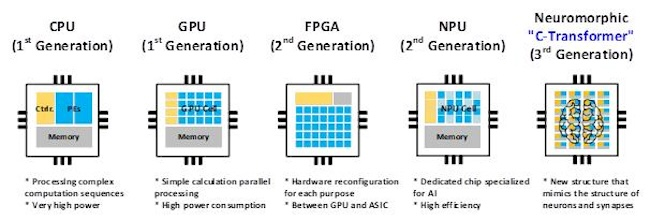
\includegraphics[width=0.8\linewidth]{images/lowpowerasic.png}
    \caption{KAIST LLM Accelerator \cite{kaist}}
    \label{fig:enter-label}
\end{figure}
\subsection{Speedup}
Im Allgemeinen werden die Leistungen in eine Metrik gegossen, damit ein objektiver Vergleich vorgenommen werden kann. Dazu entwickelte sich der allgemeine Speedup, der beschrieben wird durch: \cite{speedup}

\begin{equation}
\text{Speedup} = \frac{T_{\text{alt}}}{T_{\text{neu}}}
\end{equation}

Dabei ist:
\begin{itemize}
  \item $T_{\text{alt}}$ die Ausführungszeit vor der Optimierung bzw. der Vergleichshardware
  \item $T_{\text{neu}}$ die Ausführungszeit nach der Optimierung bzw. der Vergleichshardware
\end{itemize}
Im Folgenden wird der allgemeine Speedup verwendet, um einen Vergleich zwischen den unterschiedlichen Lastverteilungsarchitekturen aufzuzeigen.
    
    \acresetall % reset acronym counter
    %
% chapter3.tex
%

\chapter{NVIDIA Bluefield-3}
\label{cha:design}
Die im Rahmen dieser Arbeit verwendete SmartNIC ist die von Nvidia im Jahre 2022 veröffentlichte Bluefield-3. Wie bereits am Namen der Karte zu erkennen ist, handelt es sich dabei um die dritte Generation von Netzwerkkarten, die zusätzlich zur netzwerkspezifischen Architektur noch einen allgemeinen ARM-Prozessor verbaut hat. Zusätzlich wird in einem späteren Abschnitt ein Überblick über das DOCA-Framework gegeben, welches von NVidia als einheitliche Programmierschnittstelle veröffentlicht wurde, um die Programmierung der Hardware von der jeweiligen Generation unabhängig zu machen.
\section{Entstehung}
Die Entwicklung der BlueField ist ein Produkt der letzten Dekade, in der ein immerwährend größeres Interesse an der Effizienzsteigerung von Rechenzentren entstanden ist. Energiesparende Systeme, die dieselbe Leistung erreichen wie selbige Integration auf einem allgemeinen Prozessor, bieten für Systemintegratoren eine ausgezeichnete Möglichkeit, auch vor dem Hintergrund des Klimawandels energieoptimierte Systeme zu entwickeln.
\subsection{BlueField-1}
Die erste Generation der Bluefield-Hardware (siehe Abbildung 4.1) wurde im Jahre 2017 von Mellanox Technologies vorgestellt und bildet den ersten Eintrag in die Reihe der Bluefield-SmartNIC-Serie. Sie kombinierte erstmalig die ConnectX-5-Plattform mit einem ARM-basierten System-on-Chip. Die Idee dahinter war es, das Verhalten der Netzwerkplattform mittels User-Anwendungen beeinflussen zu können. Dazu wurde eine API zwischen der ConnectX und dem ARM-Prozessor entwickelt. Hierzu sei erwähnt, dass es sich bei der ConnectX-Plattform um eine bereits weit verbreitete und in viele Systeme integrierte Hardware handelte. Sie besaß bereits zum damaligen Zeitpunkt eine breite Anzahl von paketbasierten Operationen, mit deren Hilfe eine weitreichende Manipulation sowie Paket-Steering oder anderweitige Verwendungen ermöglicht wurden. Die BlueField-1 war mit einem ARM-A72 mit 4 Kernen und 8 Threads ausgestattet und besaß außerdem zwei QSFP28-Anschlüsse, welche bis zu 100 Gbps Durchsatz erreichen konnten. Die Zielgruppe der BlueField-Serie waren von Anfang an der Enterprise-Markt sowie die zahlreichen größeren Rechenzentren, in denen Rechenoperationen ausgeführt werden, die auf mehreren Computern eines Clusters oder einer Clusterstruktur ausgeführt werden. Gerade in diesem Umfeld wird eine derartige Architektur von Interesse, da der Netzwerkverkehr so anwendungsspezifischer verteilt werden und somit die Effizienz eines Rechnerverbundes steigern kann. \cite{bluefieldhistory}
\begin{figure}
    \centering
    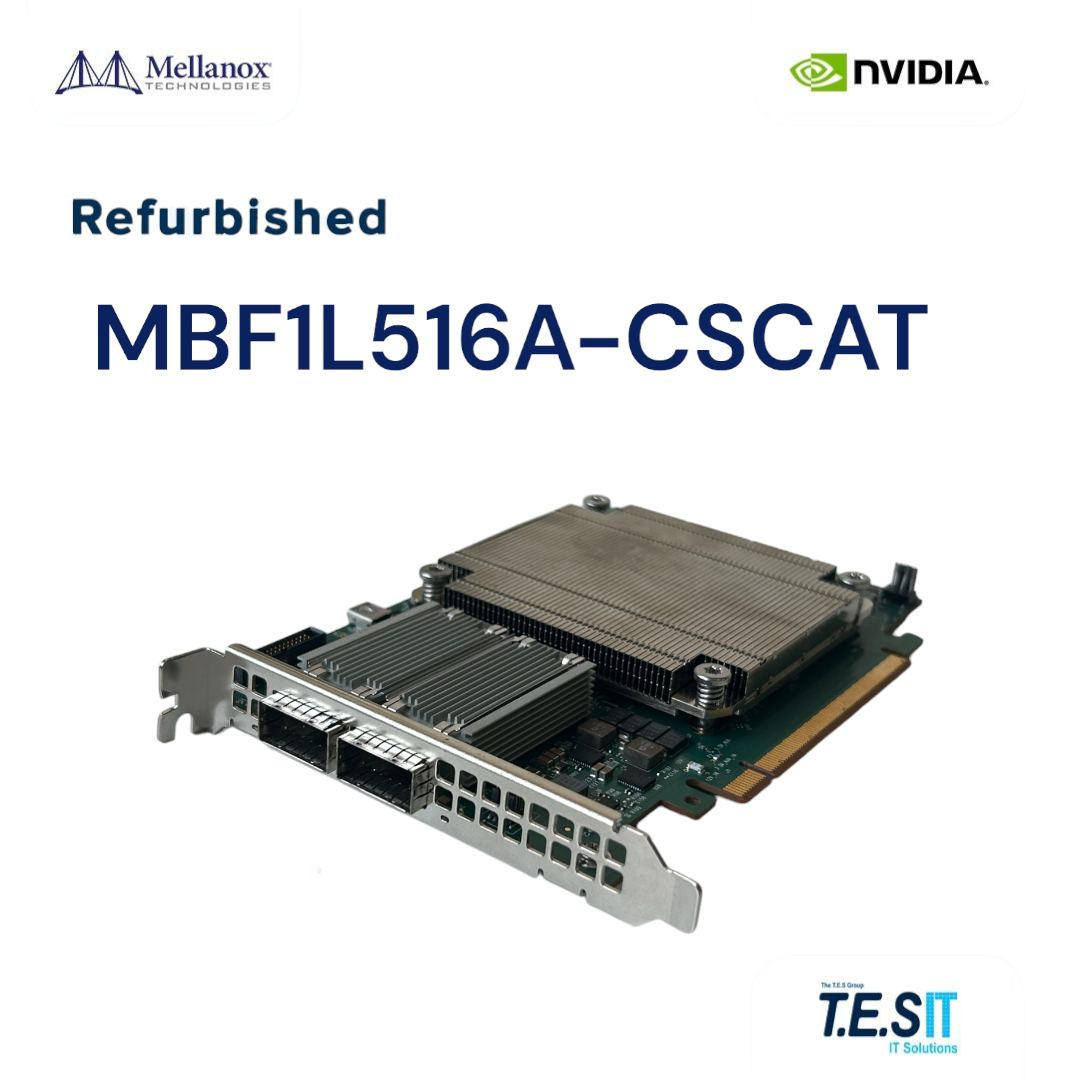
\includegraphics[width=0.65\linewidth]{images/s-l1600.png}
    \caption{BlueField-1-Karte \cite{ebay_bluefield1_2025}}
    \label{fig:enter-label}
\end{figure}
\subsection{BlueField-2}
Nach der Übernahme von Mellanox durch den Chip-Hersteller NVIDIA im Jahre 2019 wurde das Projekt BlueField von NVIDIA nicht nur weitergeführt, sondern mit dem Aufkommen von vermehrten Machine Learning Workloads sogar das Marketing ausgebaut. So wurde die BlueField-2 im Jahre 2021 unter dem neuen Hersteller NVIDIA veröffentlicht und bot nun einen QSFP56, der laut eigenem Marketing-Material bis zu 200 Gbps erreichen sollte. Abermals kam der ARM-A72 zum Einsatz, der erneut mit 4 Kernen und 8 Threads verbaut wurde. \cite{bluefieldhistory} Erstmalig wurde außerdem damit geworben, dass ein Einsatz in Machine-Learning-Rechenclustern besonders wertvoll sei. Auf Angaben, warum genau das der Fall sein sollte, wurde seitens des Herstellers verzichtet. Insbesondere nicht vor dem Hintergrund, warum es sich dabei nun um ein Alleinstellungsmerkmal anderen SmartNICs gegenüber handeln sollte.
\subsection{BlueField-3}
Zuletzt wurde im Jahre 2022 die BlueField-3 veröffentlicht, die im Rahmen dieser Arbeit zur Verwendung kam. Erstmalig wurde nun der ARM-A78 mit 8 Kernen und somit 16 Threads verbaut. Die Arbeitsspeicherarchitektur nahm zusätzlich auch den Generationensprung von DDR4 auf DDR5 vor und verwendet so einen deutlich schnelleren Speichertakt als die vorherige Generation. Außerdem wurde erneut der Netzwerkanschluss aktualisiert und verwendet nun den QSFP112. Laut NVIDIA soll mit diesem Netzwerkverbund eine Line Rate von bis zu 400 Gbps erreicht werden. \cite{battle} Dabei wird im Marketing-Material nicht explizit erwähnt, welche Paketgröße für besagten Durchsatz verwendet wurde. Erneut soll laut NVIDIA der Fokus der Hardware vermehrt auf dem Einsatz in Rechenzentren liegen, in denen größere Machine-Learning-Lasten laufen. Die BlueField-3 soll daraufhin die Rolle einer intelligenteren Paketverteilung einnehmen, wobei die Last der Lastverteilung nicht mehr auf dem Hostsystem bzw. dem entsprechenden Host-Prozessor liegt, sondern eben auf der Netzwerkkarte selbst. Außerdem sind eine Menge von weiteren speziellen hardwarebeschleunigten Hardwareeinheiten auf der neuesten Iteration der BlueField-Serie verbaut worden. Alle genannten Generationen BlueField werden per PCI-E-Stecker in den Hostsystemen verbaut und verwenden so den aktuellsten PCI-E 5.0 Standard, der auf eine theoretische Maximalbandbreite von 32 Giga Transfer/s kommt. Somit soll eine ultraschnelle Schnittstelle zwischen Hostsystem und BlueField-3 erreicht werden (siehe Abbildung 4.2).
\section{Architektur}
Um der Funktion einer intelligenten Netzwerkkarte nachzukommen, sind auf der BlueField diverse Hardwareeinheiten verbaut, die eine Reihe von Einsatzzwecken abdecken sollen. Dabei werden nicht alle angebotenen Funktionen auch tatsächlich von ASIC-Hardwareeinheiten übernommen, sondern werden teilweise komplett oder nur in bestimmten Pipelineabschnitten auf dem ARM-Core ausgelagert, um dort einer weiteren Behandlung unterzogen zu werden. Wie in Abbildung 3.2 zu erkennen ist, gliedert NVIDIA die BlueField-Karte grob in Domänen unterschiedlichster Funktion auf. Abgesehen vom ARM-Teil der Karte, womit im Wesentlichen der Bereich beschrieben wird, in dem der Prozessor, Arbeitsspeicher und restlicher I/O zusammengefasst werden, sind die beiden Bereiche \textbf{Accelerators} und \textbf{Accelerated Programmable Pipeline} diejenigen, in denen eine große Menge der eigentlichen Hardwarebeschleuniger sitzen. Allerdings geht aus dem von NVIDIA bereitgestellten Material nicht vollständig hervor, worum es sich bei dem sogenannten Datapath Accelerator handelt. \cite{nvidia_bluefield_dpu}  Im Release-Flyer der BlueField-3 steht allerdings, dass es sich dabei auch um einen Prozessor mit 16 Kernen handeln soll, der mit 256 Threads ausgestattet ist. Dies würde bedeuten, dass jeder Kern von Hause aus 16 Threads besitzt. Zusätzlich wird oft darauf verwiesen, wie einfach ein Zusammenspiel von DPU und Hostsystem mittels der PCI-E-Anbindung funktionieren soll. Im Folgenden wird eine Auswahl aus Beschleunigern und Funktionen vorgestellt, die vom Hersteller  angeboten werden. \cite{nvidia_bluefield_dpu} 
\begin{figure}
    \centering
    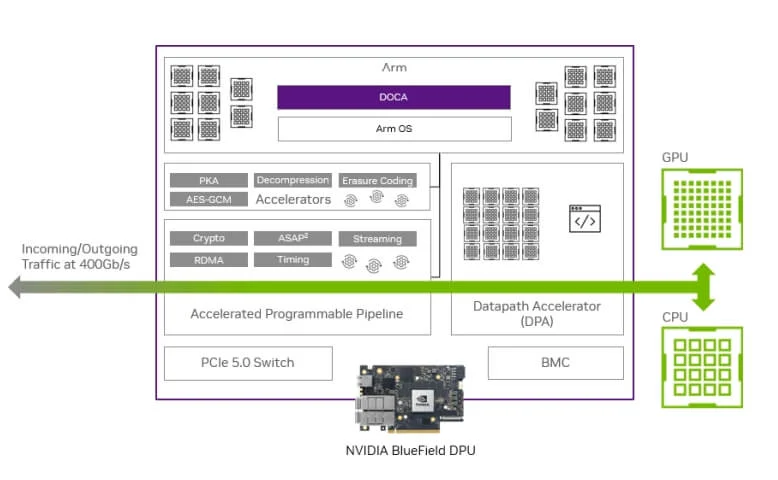
\includegraphics[width=1\linewidth]{images/nvda-bluefield-dpu.png}
    \caption{BlueField-3 Architektur}
    \label{fig:enter-label}
\end{figure}
\subsection{Hardwareeinheiten}
Im Folgenden wird eine Auswahl von Hardwarebeschleunigern vorgestellt.
\subsubsection{PKA}
PKA steht für Public-Key-Acceleration und bietet eine Reihe von Funktionalitäten im Zusammenhang mit der Arbeit mit öffentlichen Schlüsseln im Kontext von SSL-Anwendungs-fällen. So stellt es beispielsweise einfache bis komplexere arithmetische Operationen wie RSA, Diffie-Hellman sowie Addition und Subtraktion bereit. Es soll eine einfache Programmierschnittstelle bieten, sobald die DOCA-Applikation mit Verschlüsselungen hantiert, die möglichst schnell umgesetzt werden sollen.
\subsubsection{Decompression}
Die Dekompressionsbeschleuniger der BlueField-3 sollen vor allem dann zum Tragen kommen, wenn die Netzwerkkarte mit Buffern konfrontiert wird, in denen die Daten komprimiert vorliegen. Dabei soll sich diese möglichst nicht auf die Verarbeitung des Datenverkehrs auswirken.
\subsubsection{Erasure Coding}
Erasure Coding bezeichnet die Hardwareeinheit, deren hauptsächliche Funktion die Forward Error Correction ist. Dies wird dazu verwendet, um eventuelle Übertragungsfehler oder umgedrehte Bits mithilfe der Paritätsinformation reparieren zu können.
\subsubsection{AES-GCM}
Advanced-Encryption-Standard (AES) ist ein bekannter Verschlüsselungsstandard, der quasi von jedem Endgerät dieser Welt implementiert wird, um modernen Sicherheitsanforderungen gerecht zu werden. Hierzu hat NVidia eine Hardwareeinheit entwickelt, um Daten auch im eigenen Arbeitsspeicher verschlüsseln zu können.
\subsubsection{RDMA}
RDMA ist die Abkürzung für Remote Direct Memory Access. Innerhalb eines solchen Prozesses kann ein Prozess auf den Speicherbereich eines anderen Rechners zugreifen. Damit wird eine Alternative zum klassischen Netzwerkverkehr angeboten.
\subsection{Datapath Accelerator}
Der Datapath Accelerator, kurz DPA, ist für diese Arbeit von besonderem Interesse, da laut NVidia hier ein Großteil der Netzwerkverarbeitung vorgenommen wird. Wie bereits im vorherigen Kapitel zum Hardwareaufbau erwähnt, soll hier ein weiterer Prozessor zum Einsatz kommen, der über ein extremes 16-faches Multithreading verfügt. Dieses Multithreading wird benötigt, um möglichst latenzfreie Verarbeitung umzusetzen. \cite{nvidia_dpa_subsystem_2025} Leider sind seitens des Herstellers allerdings keine weiteren Angaben zur verbauten Hardware freigegeben worden. Daher ist es ohne weitere Informationen nicht möglich, die genauere Funktionsweise zu analysieren. Dennoch sollte es, sofern es sich dabei denn wirklich um den trafficverarbeitenden Prozessor handelt, in den späteren Messungen zu beobachten sein, dass der ARM-Prozessor von dem eingehenden Verkehr unberührt bleiben sollte.

\section{DOCA Framework}
DOCA ist ein von NVidia entwickeltes Framework, das speziell für die BlueField-Karten entwickelt wurde. Es gliedert sich in verschiedene Teilbereiche und unterscheidet dabei zwischen architektonischen Grundsätzen, Programmierinterfaces, aber auch dem Betriebssystem für die Karte selbst. Allgemein ist DOCA dafür gedacht, der direkte Anlaufpunkt für Entwickler zu sein, die auf der BlueField-Plattform entwickeln wollen. Damit werden auch Dinge wie Programmiersprachen, Programmierparadigmen und eine Reihe von bereits angelegten Bibliotheken bereitgestellt. Zusätzlich werden sämtliche Hardware-Treiber ebenfalls unter dem Oberbegriff DOCA zusammengefasst. \cite{nvidia_doca_framework} Im Folgenden wird ein Überblick zu DOCA im Allgemeinen gegeben und ein besonderes Augenmerk auf die für diese Arbeit relevanten Teilbereiche gelegt  (siehe Abbildung 4.3).
\begin{figure}
    \centering
    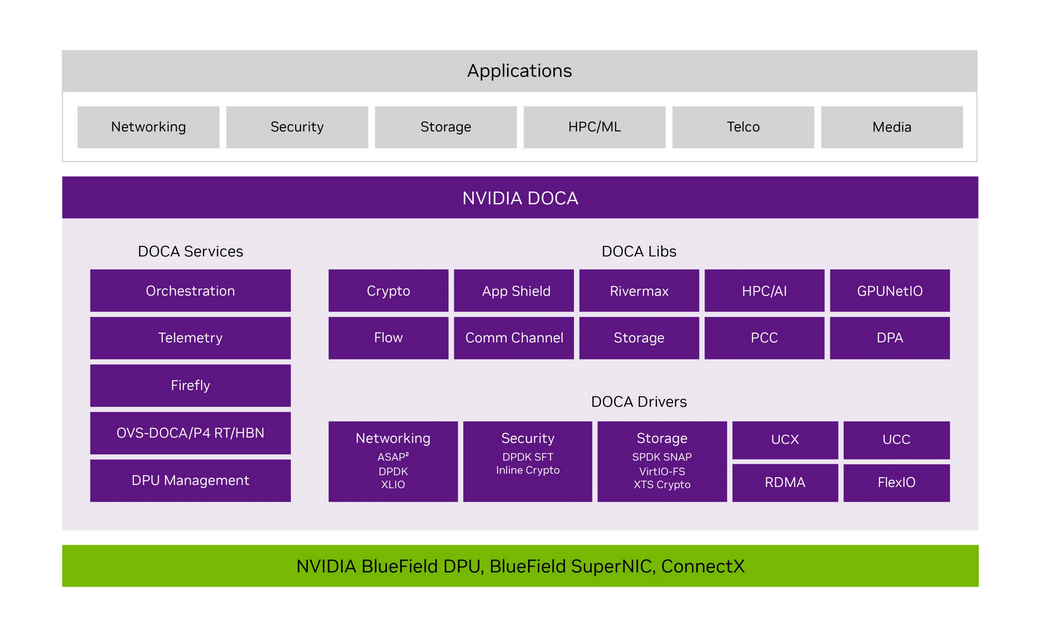
\includegraphics[width=1\linewidth]{images/Screenshot 2025-04-26 at 08-31-41 DOCA Overview - NVIDIA Docs.png}
    \caption{Überblick der Teilbereich von DOCA}
    \label{fig:enter-label}
\end{figure}
\subsection{DOCA Services}
DOCA stellt eine Reihe von Services bereit, die vorrangig dazu dienen sollen, eine Ende-zu-Ende-Lösung für einen speziellen Anwendungsfall zu bieten. Dazu gliedert NVidia diverse (Abbildung 3.3) Unterkategorien aus. Einerseits aufgrund des primären Anwendungsfeldes in Rechenzentren wird viel Wert auf Orchestrierung gelegt. Leider bleibt NVidia hier bemerkenswert ungenau, was genau damit eigentlich gemeint ist. Bei der Telemetrie hingegen stellt NVidia eine große Schnittstelle bereit, um genaue hardwarebezogene Daten abrufen zu können. Hierzu werden den Entwickelnden zwei Tools bereitgestellt. Das Tool \textbf{doca\_telemetry\_diag} stellt die Konfiguration des Loggings dar. Dazu kann mithilfe besagter Tools festgelegt werden, welche Telemetriedaten und auch in welchem Samplingintervall erhoben werden sollen. Diese Daten können dann in diversen auswählbaren Dateiformaten abgerufen werden. \textbf{doca\_telemtery\_pcc} soll den Zugang zu speziellen algorithmischen Daten ermöglichen. Damit sind die bereits in DOCA vorimplementierten Funktionen gemeint, die meist hardwarebeschleunigt, also außerhalb des sichtbaren Bereichs des ARM-Hosts, ausgeführt werden. Sonstige Services wie beispielsweise der Firefly sind NVidias Implementierungen des Precision Time Protocols. Ziel dieses Protokolls ist es, die Zeit innerhalb eines Clusters möglichst genau propagieren zu können. Dazu verspricht NVidia, möglichst viel von dieser Komplexität vor dem Anwender mithilfe von Firefly fernzuhalten. Außerdem setzt NVidia zur Konfiguration des Datenverkehrs stark auf die Integration von Open vSwitch (OVS). Dazu wurde eigens ein eigener Service entwickelt, der abermals die eigentliche Komplexität des Konfigurationsprozesses dem Entwickler abgenommen werden soll. Hauptgrund ist allerdings vermutlich, dass, um mit den spezifischen Hardwareeinheiten überhaupt kommunizieren zu können, die Open vSwitch-Interfaces angepasst werden müssen. 
\subsection{DOCA Bibliotheken}
Damit eine reibungslose Inbetriebnahme sowie Programmierung einer SmartNIC erfolgen kann, muss klar definiert sein, wie, sofern programmatische Konfigurationen erfolgen sollen, ein Entwickler mit der entsprechenden Hardwareeinheit kommunizieren kann. Damit ist es nicht mehr nötig, die Feinheiten der einzelnen Hardwarekommunikationskanäle zu implementieren, sondern es kann auf eine mehr oder weniger vereinheitlichte Programmierschnittstelle zugegriffen werden. Dazu stellt NVidia Programmbibliotheken in Form von C-Headern bereit, mithilfe derer intrinsische Funktionen auf der Architektur ausgeführt werden können. Dabei lässt sich grob formulieren, dass jede in Kapitel 3.2.1 genannte Hardwareeinheit eben auch eine entsprechende Bibliothek bekommen hat. Zusätzlich gibt es aber auch Bibliotheken, die Funktionen wie Speicherverarbeitung für Anwendungsfälle wie verteilte Speichersysteme implementieren.
\subsection{DOCA Flow}
DOCA Flow ist die Bibliothek, die die Verarbeitung und Modifikation von Netzwerkpaketen enthält. Das Versprechen seitens NVidia ist hierbei, dass alle Funktionen von Flow auf den Hardwarebeschleunigern ausgeführt werden können. DOCA Flow wird, wie viele moderne Systeme, deklarativ programmiert. Das bedeutet, der State des aktuellen Netzwerkverkehrs ist immer genau so, wie er durch die Konfiguration deklariert wurde. Dies hat den großen Vorteil, dass die Entwicklung und in der Folge auch das Debugging sich immer direkt mit dem Programmcode selbst befassen kann, da keine Fehler zur Laufzeit entstehen können (sollten) die so nicht klar vorher definiert worden sind.
Allgemein ist DOCA Flow darauf ausgelegt, statt Pakete einzeln zu behandeln, in Netzwerkdatenpfaden den Verkehr zu steuern. Dazu werden die Hardwareregeln wie beispielsweise \textbf{Packet Matching}, \textbf{Forwarding} und \textbf{Monitoring} definiert. Beim Packet Matching wird ein Zusammenspiel aus Filter- und Match-Regeln verwendet, um Pakete aus dem Datenfluss der NIC auszuwählen und der entsprechenden Pipe zuzuordnen (siehe Abbildung 4.4). \cite{nvidia_doca_flow_2025}
\subsubsection{Flow Pipe}
\begin{figure}
    \centering
    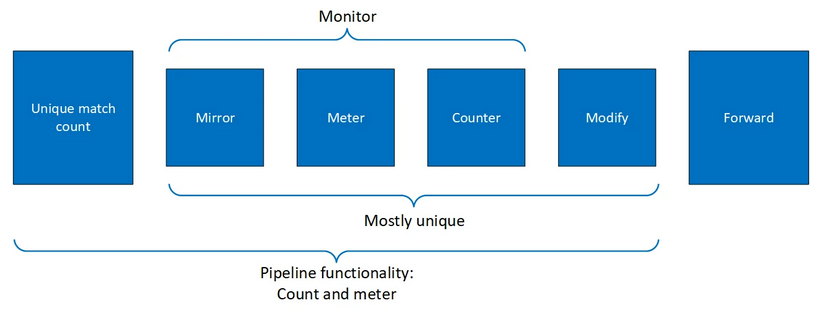
\includegraphics[width=1\linewidth]{images/pipe.png}
    \caption{Schemata und Zugehörigkeiten einer Flow Pipe}
    \label{fig:enter-label}
\end{figure}
Eine Flow Pipe beschreibt einen genannten Datenpfad, der deklarativ an die BlueField-3 API übergeben wird. Dabei setzt sich eine Flow Pipe immer aus den vier wesentlichen Bestandteilen \textbf{Match}, \textbf{Monitor}, \textbf{Action} und \textbf{Forward} zusammen. Diese Bestandteile können in \textbf{Entries} organisiert werden. Sie bilden die tatsächlichen aktiven Teile der Pipe. Pipes bilden eine Abstraktion eines Datenpfades, auf denen die einzelnen Entries angewendet werden.

Beim Match wird mithilfe einer Zusammensetzung aus Filtern und Match-Regeln klar definiert, welche Pakete aus dem Datenstrom der BlueField genommen werden sollen und welcher entsprechenden Pipe zugeordnet werden. 

Daraufhin wird das Paket laut Dokumentation gespiegelt und dem Monitorteil übergeben. Dieser erlaubt es, Daten über die Pipe auszulesen. So kann zur Laufzeit die Anzahl der von der Pipe verarbeiteten Pakete sowie deren Größe in Bytes ausgelesen werden. Im Verlauf der Messung im späteren Teil wurde der Versuch durchgeführt, ob ein ein- bzw. ausgeschaltetes Monitoring Auswirkungen auf die Leistungsfähigkeit der Karte hat. Dies ist klar zu verneinen. Weder Bandbreite noch Pakete/Sekunde wurden von dem Monitoring beeinflusst.

Nachdem nun Pakete in der entsprechenden Flow Pipe ankommen, können nun eine Reihe von Aktionen auf diese ausgeführt werden. Diese Funktionen werden in Entries durchgeführt. Darunter befinden sich vor allem Funktionen, die die Ethernet- sowie IP-Header modifizieren können. Es ist so beispielsweise nicht ohne weiteres möglich, Pakete einzeln zu verarbeiten, sondern nur Klassen von Paketen, die eben in der entsprechenden Pipe bzw. dem entsprechenden Entry angekommen sind. Die eigentliche Payload des Paketes kann \textbf{nicht} von Flow verarbeitet werden. Dies ist vor allem der Tatsache geschuldet, dass es sich hierbei eben um die Programmierung von Hardwarebeschleunigern handelt. Würden wir Pakete einzeln verarbeiten wollen, so müssten diese zur Laufzeit auf den Prozessor der SmartNIC gebracht werden, was mit erheblichen Leistungseinbußen einhergehen würde.
Die Payload der Pakete kann nicht verarbeitet werden, da diese eine variable Länge besitzen kann, was ein Problem für eine feste Hardwarearchitektur darstellt. Bei festgelegten Header-Bitfeldern allerdings kann eine festdefinierte ASIC-Hardware gut die entsprechenden Bits mithilfe von einfachen logischen Bauteilen verarbeiten (siehe Abbildung 4.5).  \cite{nvidia_doca_flow_v1_2} 
\begin{figure}
    \centering
    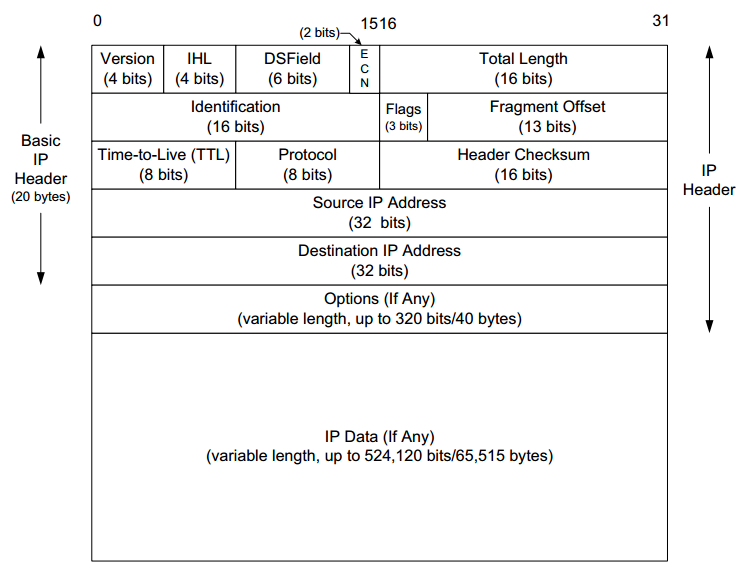
\includegraphics[width=0.8\linewidth]{images/figure_5-1.png}
    \caption{Aufbau eines IP-Headers}
    \label{fig:enter-label}
\end{figure}
In Abbildung 4.5 ist zu erkennen, dass sich bestimmte Teile eines Headers immer an genau der gleichen Stelle im Bitfeld befinden. So muss die Hardware nicht erst parsen bzw. erkennen, wo im Paket sich welche Daten befinden.

Zuletzt kann in einer Pipe aber auch in den Entries selbst mittels des \textbf{Forward} festgelegt werden, wohin die relevanten Pakete geleitet werden sollen. Dabei kann sowohl direkt auf einen Port, der einem entsprechenden Hardware-Port auf der Karte gleicht, eine andere Pipe oder gar kein Folgeziel gewählt werden. Bei letzterem handelt es sich logisch um einen Drop des Pakets. Von besonderem Interesse ist allerdings die Funktion, in eine andere Pipe weiterzuleiten, da sich so komplexere Anwendungen umsetzen lassen, in denen einzelne Pipes bestimmten Traffic verarbeiten und mehrere Datenströme modifiziert werden können. Allgemein bietet DOCA Flow die Kategorisierung dieser Pipes. Dabei wird zwischen sogenannten \textbf{Steering Domains} unterschieden. Diese verbieten gewissen Pipefunktionen, wenn der entsprechenden Domain eine Pipe hinzugefügt wurde. 
\begin{figure}
    \centering
    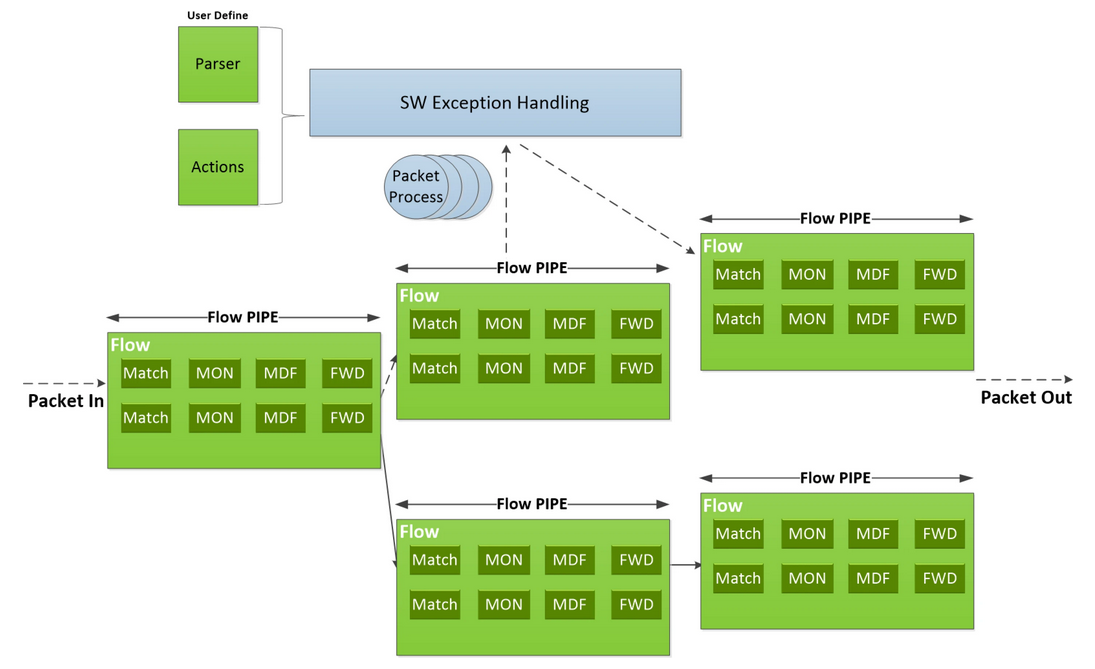
\includegraphics[width=1\linewidth]{images/Screenshot 2025-04-30 at 11-16-05 DOCA Flow - NVIDIA Docs.png}
    \caption{Beispielhafter Flow-Pipe-Aufbau}
    \label{fig:enter-label}
\end{figure}

In Abbildung 4.6 ist eine Beispielanwendung per Diagramm zu sehen, in der eine Verkettung von Flow Pipes erfolgt ist. Es ist auch möglich, dass, wenn Pakete nicht von einer entsprechenden Pipe gefangen werden, sie an einen Hostkern durchgereicht werden. Dort kann dann ein weiteres Programm laufen, welches daraufhin diese Pakete verarbeitet. Dabei verlässt das Paket allerdings den hardwarebeschleunigten Bereich und ist wieder an die Performance des ARM-Cores gebunden.
\subsubsection{Flow Entry}
\begin{figure}
    \centering
    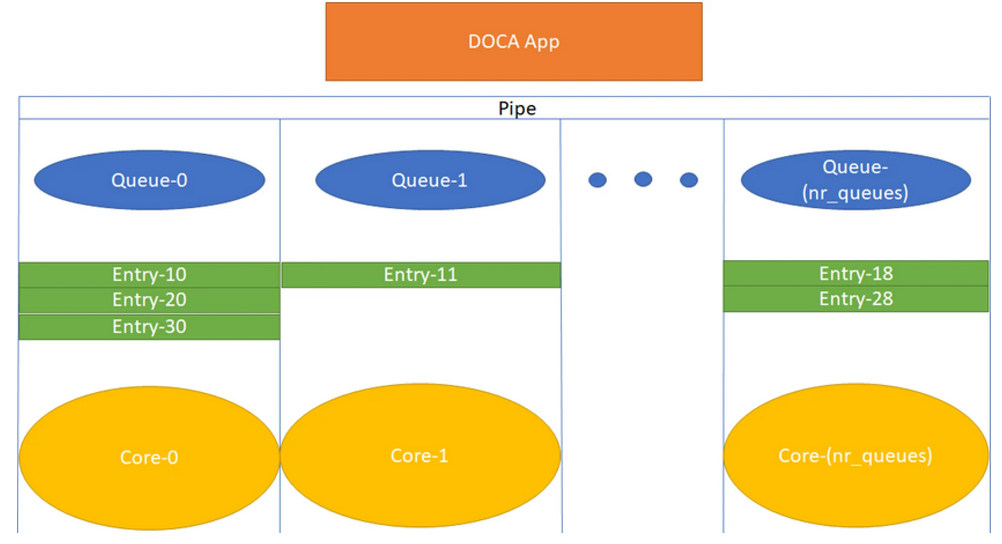
\includegraphics[width=1\linewidth]{images/entries.png}
    \caption{Auslagerung von Pipe Entries}
    \label{fig:enter-label}
\end{figure}
Laut NVidia werden Entries einer Flow Pipe auf mehreren Kernen des Data Accelerators verarbeitet. Jedem dieser Kerne ist eine entsprechende Queue mit den zu verarbeitenden Paketen zugeordnet  (siehe Abbildung 4.7). Durch diese Parallelisierung soll es möglich sein, dass der Paketverkehr ohne Latenzzugewinn verarbeitet werden kann. Leider waren im Rahmen dieser Arbeit keine weiteren Daten, wie genau diese Lastverteilung auf den 256 Threads funktioniert, auffindbar. Flow Entries können spezielle Aufgaben für eine Pipe übernehmen. So werden beispielsweise in XenoFlow die Entries genutzt, um pro Entry an ein bestimmtes Backend weiterzuleiten. Entries sind allerdings lose an die Pipe-Definitionen gebunden. Soll beispielsweise in einem Entry entschieden werden, ob an Port 0 oder Port 1 weitergeleitet werden soll, so muss in der Pipe das entsprechende Forward-Feld auf 0xffff gesetzt sein, damit die Hardware weiß, dass der Forwardschritt erst im Entry erfolgt. Selbiges gilt natürlich für Matching und Actions.
\subsubsection{Packet Matching}
Für die Funktion eines Lastverteilers ist eine der Hauptfunktionen, den gesamten Traffic in handhabbarere Teillasten zu modulieren, damit diese dann auf verschiedene Backends verteilt werden können. Dazu ist eine Art des Packet Matchings besonders praktisch. 
\begin{figure}
    \centering
    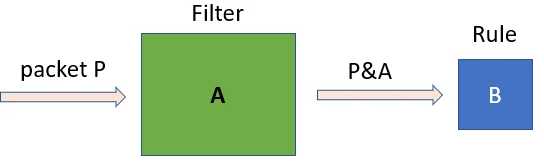
\includegraphics[width=1\linewidth]{images/paketmatchng.png}
    \caption{Matching Schema der BlueField}
    \label{fig:enter-label}
\end{figure}
Das Packet-Matching aus DOCA Flow ist in Abbildung 4.8 zu sehen. Zunächst erreicht ein Paket den Filter und wird mit diesem auf der Bit-Ebene verundet. Sprich, das Ausgabebitfeld besitzt an einer Position eine 1, wenn das Datenpaket und der Filter an der gegebenen Stelle auch eine 1 gesetzt haben. So kann eine Art Vorauswahl realisiert werden, in der Entwickler festlegen können, welche Bits des entsprechenden Feldes überhaupt analysiert werden sollen. Daraufhin erreicht das neu berechnete Bitfeld die Regel. In dieser wird überprüft, ob das Bitfeld der Regel entspricht. Wenn dies der Fall ist, so wird das Paket dem Match zugeordnet. Wird die Regel nicht erfüllt, wird das Paket fortan als Miss betrachtet.
\begin{itemize}
  \item Sei $P \in \{0,1\}^n$ das eingehende Paket als Bitfeld.
  \item Sei $F \in \{0,1\}^n$ das Bitfeld gibt als Maske an welche Bits berücksichtigt werden sollen
  \item Die bitweise Filterung erfolgt durch eine Konjunktion  
  \[
    P_{neu} = P \land F = (P_1 \land F_1, P_2 \land F_2, \dots, P_n \land F_n)
  \]
  \item Sei $R \in \{0,1\}^n$ das Bitmuster der Rule. Ein Paket wird als \emph{Match} klassifiziert, wenn gilt:
  \[
    P_{neu} = R
  \]
  \item Sonst wird das Paket als \emph{Miss} behandelt:
  \[
    P_{neu} \ne R
  \]
\end{itemize}

In der Matching-Deklaration kann außerdem unterschieden werden, ob Pakete explizit oder implizit gematcht werden sollen. Damit kann festgelegt werden, ob wir wie beim expliziten Match das genaue Bitfeld aus dem Datenfluss extrahieren wollen. Alternativ können wir mittels des impliziten Matchens Muster aus den Bitfeldern extrahieren. Sogleich können mehrere Bitfelder extrahiert werden, sofern diese die deklarierten Muster enthalten.


Sobald Bitfelder allgemein verarbeitet werden sollen, so muss dies mithilfe eines C Structs klar definiert werden. Dazu werden alle Bits des gewünschten Bitfeldes beim Definieren der Datenstruktur zunächst auf 1 gesetzt.
In XenoFlow sieht eine Filter-Implementierung, die alle IP-Adressen in Gerade- und Ungerade-Klassen teilt, wie folgt aus:
\begin{minted}{c}
match.outer.ip4.src_ip = BE_IPV4_ADDR(255, 255, 255, 255);
match_mask.outer.ip4.src_ip = BE_IPV4_ADDR(0, 0, 0, 1);
\end{minted}
Somit ist die Match-Maske aktiviert. Dies bedeutet, dass wir nun nicht auf exakte Bitfelder matchen, sondern mittels der Match-Maske Bitmuster deklarieren können, die wir dann in den Entries matchen können. Das bedeutet, nur allein die Match-Maske in der Pipe führt noch nicht zu Paketen, die gematcht werden. Es bedarf in der gezeigten Konfiguration immer noch eines speziellen Matches im Entry wie folgt: 
\begin{minted}{c}
match.outer.ip4.src_ip = BE_IPV4_ADDR(0, 0, 0, 1);
\end{minted}
Die Kombination aus Pipe-Match und Entry-Match würde nun alle Pakete dem Entry zuordnen, die eine IP-Adresse haben, deren Quell-IP am letzten Bit eine 1 gesetzt hat.
\subsection{DOCA Treiber}
Damit die entsprechenden Hardwareeinheiten vom ARM-SmartNIC-System aus betrieben werden können, hat NVidia eigens bestimmte Treiber entwickelt. Dazu zählt unter anderem auch eine DPDK-Implementierung. DPDK steht für Data Plane Development Kit und ist ein von der Linux Foundation verwaltetes Open Source Projekt. Es wird verwendet, um Kernelprozesse der Datenverarbeitung aus dem Linuxkernel in den Userspace zu verlagern, um dort eine Verarbeitung vorzunehmen. DOCA Flow nutzt somit DPDK, um die Pakete von dem Data Accelerator auf den ARM-Kern in den Userspace zu bringen, da DOCA Applikationen im Userspace ausgeführt werden. 

Außerdem hat NVidia in DOCA andere Treiber entwickelt, wie beispielsweise Virtio-FS, mithilfe derer eine kompakte Integration von Dateisystemen in die BlueField-Systeme vorgenommen werden kann. Ein denkbarer Einsatzzweck wäre die dynamische Anbindung von Persistent Volumes in einem Kubernetes-Cluster, sofern sich die Volumes auf einem anderen Knoten befinden als der Pod, der versucht, das entsprechende Persistent Volume zu claimen.
\subsection{Anwendungen}
DOCA stellt eine Reihe von bereits implementierten Applikationen bereit, die eine Reihe von denkbaren Anwendungszwecken von DOCA präsentieren sollen. Im Rahmen dieser Arbeit wurden drei dieser Applikationen näher betrachtet.

\textit{So ist in einem Flyer auch von einem Load Balancer die Rede. Allerdings war dieser nicht auffindbar.}

\subsubsection{Firewall}
Hier hat NVidia eine beispielhafte Firewall-Applikation entwickelt, deren Sinn und Zweck es ist, mit Hilfe von gRPCs zwischen Host und SmartNIC dynamisch Hardwareregeln hinzuzufügen bzw. diese wieder zu entfernen. Dabei wird der Host von dieser Aufgabe entlastet und die Pakete werden nicht erst auf dem Zielsystem, sondern bereits auf deren Netzwerkkarten verworfen.

\subsubsection{GPU Packet Processing}
Sollte im Hostsystem zusätzlich zur BlueField auch noch eine GPU verbaut sein, so bietet DOCA eine Applikation an, mit deren Hilfe Pakete von der GPU verarbeitet werden können. Das könnte beispielsweise für Anwendungen sehr nützlich sein, in denen nicht nur Header-Bitfelder verarbeitet werden, sondern auch die Payloads der Pakete verarbeitet werden sollen. Dazu eignen sich die Vektoreinheiten einer Grafikkarte gut, da diese auf hochdimensionale Vektorräume ausgelegt sind. 

\subsubsection{Switch}
Die Kommunikation zwischen Host-System und der DPU wird mittels verschiedener Hardware-Networking-Interfaces angeboten. Bei der Switch-Applikation wird der Netzwerkverkehr auf der DPU in verschiedene Teilverkehre gespaltet und dann auf mehrere dieser Networking-Interfaces weitergegeben. Dadurch wird abermals das Hostsystem entlastet, da die spezielle Fallunterscheidung eines jeden Pakets nicht mehr vom Prozessor des Hosts übernommen werden muss, sondern bereits auf der Netzwerkkarte passiert. Außerdem bietet die SmartNIC-Architektur zusätzlich die Möglichkeit, bestimmte Hardwarebeschleuniger für diesen Einsatzzweck zu verwenden.
    
    \acresetall % reset acronym counter
    \chapter{Netzwerklastverteilung}
\begin{figure}
    \centering
    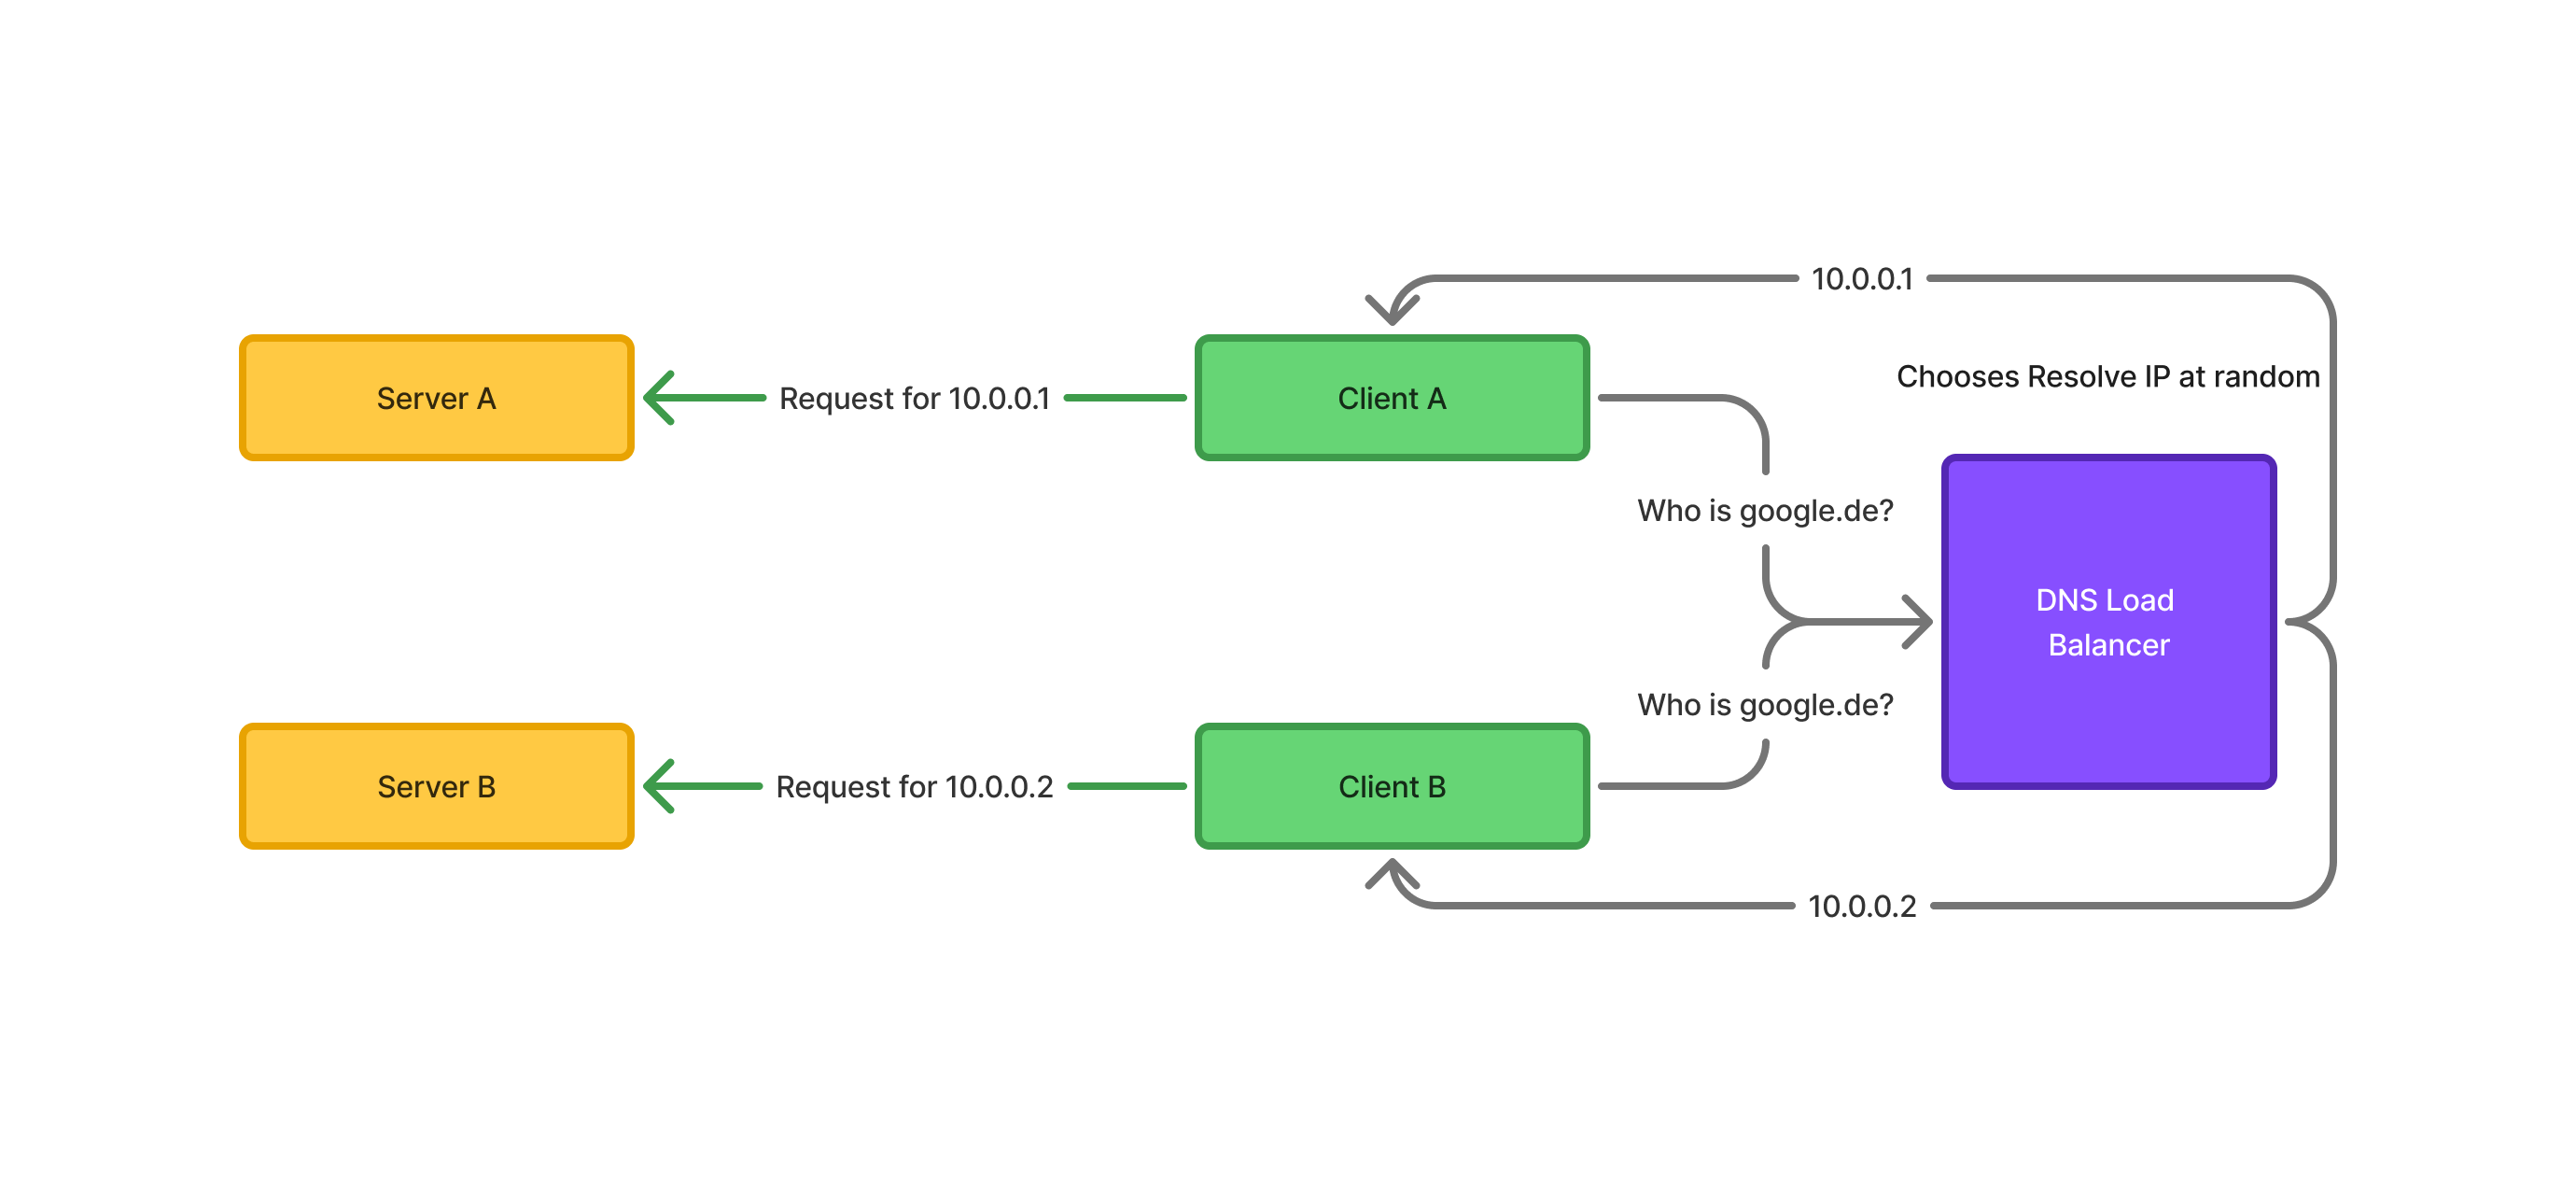
\includegraphics[width=1.1\linewidth]{images/DNS Loadbalancer(1).png}
    \caption{Aufbau eines DNS Loadbalancers}
    \label{fig:enter-label}
\end{figure}
Lastverteilung spielt in der Computerwissenschaft eine sehr wichtige Rolle. Das Problem wird immer dann interessant, wenn ein Computersystem an seine Grenzen der Bearbeitbarkeit gebracht wird. So wird auch bei Mehrkernprozessoren ein Algorithmus derart aufgeteilt, dass jeder Kern ein Teilproblem löst, welches nach Fertigstellung des Teilproblems mit den Ergebnissen der anderen Kerne zusammengesetzt wird. So lässt sich in vielen Fällen ein sehr bedeutender Speedup für bestimmte Algorithmen erreichen, indem der Algorithmus auf mehrere Recheneinheiten verteilt wird. \cite{lbtheory}

Betrachten wir nun Computerarchitekturen in Netzwerkumgebungen, so bilden wir eine Abstraktionsebene über den Mehrkernprozessoren. Nun ist es nicht mehr nur von Interesse, wie ein einzelner Prozessor das theoretische Problem bearbeitet, sondern es muss vielmehr betrachtet werden, wie sich besagtes Problem in einem Netzwerk aus Computern verhält. Mit dem Aufkommen des zivil und populär verfügbaren Internetanschlusses in den 90er Jahren ist vor allem die netzwerkbasierte Lastverteilung relevant. Die Kapazität eines einzelnen Computers, die Anfragen von Nutzern aus dem Internet zu verarbeiten, ist schnell erreichbar, sobald die Nachfrage auf Nutzerseite groß ist. So entstanden alsbald in den 90ern Ideen, wie es dennoch möglich ist, hochskalierende Anfrageraten zu beantworten. 

Da im Rahmen dieser Arbeit ein L3/L4-Lastverteiler implementiert wird, werden im Folgenden die historischen wie aktuellen Ansätze für Lastverteilung auf diesen Schichten behandelt.

\section{Entstehung}

Wie bereits erwähnt, ist mit dem Aufkommen des Internets parallel das Interesse an Möglichkeiten der Lastverteilung gestiegen. Noch bevor dazu dedizierte Maschinen oder Anwendungen entwickelt wurden, gab es Ansätze, das Problem zu lösen. Dabei wurde der Aufbau des DNS-Systems genutzt. Wenn eine bestimmte URL von einem Client-Rechner angefordert wird, so wird zunächst eine Anfrage, in der die gesuchte URL steht, an einen DNS-Server geschickt. Dieser schlägt daraufhin nach, ob ihm die URL bekannt ist. Sollte dies der Fall sein, so schickt er ein Paket mit der entsprechenden IP-Adresse zurück an den Client-Rechner. \cite{hong2006dns} Dabei lässt sich nun auf ganz einfache Art und Weise die Last verteilen. Der DNS-Server hat, wie in Abbildung 5.1 zu sehen, nicht nur eine IP-Adresse für einen Server hinterlegt, sondern mehrere, aus denen er nun aus einem eigens dafür implementierten Algorithmus wählen kann, welche IP an den Client zurückgesendet wird. So konnte damals bereits mit einfachen Mitteln Last verteilt werden. 

Allerdings bringt dieser Ansatz natürlich eine Reihe von Problemen mit sich. So kann der DNS-Server den aktuellen Status der Backend-Server nicht kennen. Sollte einer der Backend-Server offline sein, so wird weiterhin seine IP an die Clients gesendet und somit als funktionierendes Backend propagiert. Außerdem lässt ein DNS-Server keine intelligente Lastverteilung zu. Bei dieser verbesserten Form der Lastverteilung werden die Prozessorauslastung, Speichernutzung oder anderweitige Ressourcenstatistiken verwendet, um eine Entscheidung darüber zu fällen, welches Backend noch weitere Anfragen bearbeiten kann. Außerdem müsste der Client den entsprechenden DNS-Server standardmäßig konfiguriert haben. Dies ist aber nicht zwingend gewährleistet.

\section{Hardwarelastverteiler}
Zum Ende der 90er Jahre hin zum Beginn der 2000er entwickelten eine Reihe von Herstellern hardwarebasierte Lastverteilungslösungen. Nennenswerte Hersteller sind hierbei F5-Networks mit \textbf{BIG-IP} (siehe Abbildung 5.2) aber auch Cisco oder Citrix. Bei diesen Geräten kamen auch erstmalig ASICs zum Einsatz. Grund dafür war die Tatsache, dass damalige Prozessoren bei weitem nicht schnell genug waren, um große Datenströme zu verarbeiten. Außerdem boten die damaligen Geräte zusätzliche Funktionalitäten an. Darunter waren grafische Nutzeroberflächen oder integrierte Backend Health Checks. \cite{bigip} Die damaligen ASICs fokussierten sich damals vor allem auf L4-Paket-Forwarding. Außerdem wurden derartige Geräte meist als eine Art Komplettlösung für sämtliche Aufgaben des Datenverkehrs vermarktet. So wurde auf selbigen Geräten meistens eine Firewall mit angeboten, wodurch auch sicherheitstechnische Funktionen wie Distributed Denial of Service Attacken bekämpft werden konnten. All diese Funktionen konnten mithilfe von Logging untersucht und analysiert werden. Außerdem konnten einige Hardwarelastverteiler auch an Anwendungen angepasst werden, sodass zusätzlich eine L7-Lastverteilung möglich wurde.
\begin{figure}
    \centering
    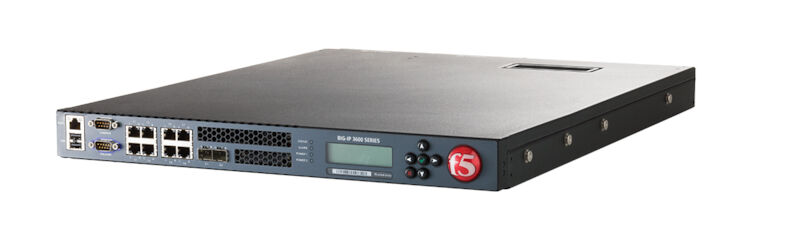
\includegraphics[width=1\linewidth]{images/s-l1600.jpg}
    \caption{BIG-IP von F5-Networks \cite{wtit_bigip_5000_series}}
    \label{fig:enter-label}
\end{figure}
\section{Softwarelastverteiler}
Softwarelastverteiler unterscheiden sich deutlich von den Hardwarelastverteilern in dem Punkt, dass bei softwarebasierter Lastverteilung keine spezialisierte Hardware in Form von ASICs oder FPGAs zum Einsatz kommt. Es werden lediglich Programme auf Servern ausgeführt, deren Funktion es ist, den Netzwerkverkehr zu steuern. Wie im vorherigen Absatz beschrieben, ist dies nur aufgrund der Entwicklungen im Bereich der Hardware der letzten zwei Jahrzehnte möglich geworden. Während dieser Zeit wurden gängige Prozessoren nicht nur um Rechenkerne erweitert, sondern erhielten außerdem größeren Cache und schnellere Anbindungen an sonstige Ein- und Ausgabeeinheiten. Außerdem lassen sich softwarebasierte Lastverteiler deutlich besser in moderne, meist VM-betriebene Netzwerkumgebungen integrieren. Die Natur eines anwendungsbasierten Lastverteilers bietet die Möglichkeit, genaue anwendungsfallspezifische Modifikationen vorzunehmen, womit eine kompakte Integration in ein System vorgenommen werden kann. \cite{softwarelb} So entstanden eine Menge von nennenswerten Anwendungen, die sich eine Lösung von softwarebasierter Lastverteilung zum Ziel gesetzt haben. Die wohl bekanntesten aktuellen Vertreter dieser Klasse sind Programme wie HAProxy, Nginx und mod\_proxy von Apache. \cite{soni2016load} Alle diese sind allerdings Lastverteiler der Klasse L7 und somit Userspace-Lastverteiler. Außerdem ist ebenfalls an der Universität Potsdam im Rahmen der Masterarbeit von Phillip Ungrund der Katran-Lastverteiler in einem ähnlichen Testszenario untersucht worden. Diese Messreihe ist sehr gut mit dem XenoFlow vergleichbar, da in Phillip Ungrunds Messungen ebenfalls DNS-Pakete verwendet wurden \cite{ungrund}. 
\section{Kubernetes und Userspace Load Balancer}
Kubernetes ist eine moderne Container-Runtime, welche im Gegensatz zu klassischem Docker oder Podman nicht nur auf einem Rechner laufen kann, sondern gleich eine Netzwerkabstraktion mit sich bringt. In dieser werden mehrere Computer zu einem Kubernetes-Cluster zusammengefasst und können mittels dedizierter Control-Plane-Knoten kontrolliert werden. In solch einer Umgebung wird fast vollständig über REST-APIs kommuniziert. Anwendungen werden in solch einem Cluster in feingranulare Microservices heruntergebrochen. Ziel eines solchen Ansatzes ist es, die Teile eines komplexen Systems einzeln wartbar zu machen, aber auch Skalierfähigkeit zu erhalten. Grundsätzlich wird in Kubernetes-Clustern stets empfohlen, den einzelnen Microservices möglichst wenig State zu geben. Damit soll garantiert werden, dass die Provisionierung von Kubernetes übernommen werden kann. Dinge wie Replikas und redundante Anwendungen können so von Kubernetes bereitgestellt werden. \cite{vasireddy2023kubernetes}

In besagter Kubernetes-Architektur werden Ressourcen typisiert. So werden Container in Ressourcen vom Typ \textbf{Pod} ausgeführt. Diese sind meistens ebenfalls ein Teil einer abstrakteren Ressource namens \textbf{Deployment}, in der mehrere Pods zusammengefasst werden können. Damit nun ein solches Deployment von außerhalb des Kubernetes Clusters erreichbar ist, muss eine Ressource vom Typ \textbf{Service} definiert werden. Solch ein Service kann wiederum unterschiedliche Arten haben. Ist die Art des Services \textbf{LoadBalancer} so wird an einen eventuellen Cloud Provider wie GKE (Google), AWS (Amazon) oder Azure (Microsoft) kommuniziert, dass eine Lastverteilungs-IP-Adresse bereitgestellt werden soll, die auf den verknüpften Service zeigen soll. Dieser Service zeigt wiederum auf das Deployment, in dem entsprechend der gesuchte Endpunkt für die Kommunikation liegt. Der im Rahmen dieser Arbeit implementierte Load Balancer eignet sich in einem solchen Szenario sehr gut, da er auf der Netzwerkkarte des Providers in den für die Lastverteilung bestimmten Servern ausgeführt werden kann. 
\subsection{Lastverteilung auf einer Data Processing Unit (DPU)}
DPUs bieten eine weitere Plattform für Hardwarelastverteiler, die zu den jüngsten Vertretern dieser Klasse zählen. Wie in Abbildung 5.3 zu sehen, werden bei dieser Art von Architektur die Netzwerkkarten mit ihren entsprechenden (hier rot markierten) Hardwarebeschleunigern selbst zur Lastverteilung verwendet. So kann gänzlich auf einen separaten Lastverteilungsknoten verzichtet werden.
\begin{figure}
    \centering
    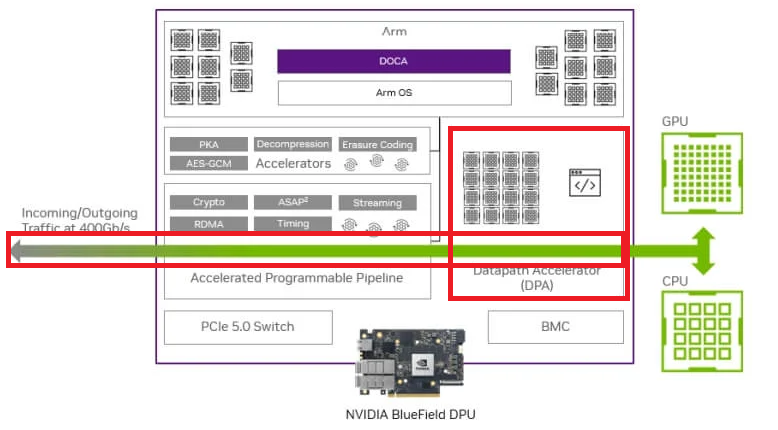
\includegraphics[width=0.9\linewidth]{images/nvda-bluefield-dpu-red.png}
    \caption{Für Hardwarelastverteiler relevante Bereich auf einer DPU \cite{fibermall_bluefield3}}
    \label{fig:enter-label}
\end{figure}
    
    \acresetall % reset acronym counter
    \chapter{XenoFlow Loadbalancer}
\label{cha:implementation}
Ziel dieser Bachelorarbeit war es, einen möglichst hardwarebeschleunigten Lastverteiler zu entwickeln. Dazu wurde das DOCA Flow Framework verwendet, da die zur Verfügung stehende Netzwerkkarte eine BlueField-3 ist. Im folgenden Kapitel wird ein Überblick über die Entwicklung mit DOCA Flow gegeben und es werden die Kernelemente des XenoFlow LoadBalancers vorgestellt. XenoFlow ist nicht für Produktionsumgebungen gedacht, sondern soll vielmehr ein Proof-of-Concept darstellen und einen speziellen Anwendungsfall demonstrieren. XenoFlow ist aktuell auch nur in der Lage, UDP-Pakete zu verarbeiten. Diese Entscheidung ist damit zu begründen, dass eine beispielsweise eine TCP-Verbindung mehr Umstände beinhaltet, die berücksichtigt werden müssten. Zunächst soll aber nur die Machbarkeit und die allgemeine Performance beurteilt werden. Der komplette Quellcode von XenoFlow ist unter der MIT veröffentlicht und unter den weiter unten angegebenen Git-Repositories verfügbar.
\section{Entwicklung}
NVidia stellt eine Menge von Beispielapplikationen für die verschiedenen DOCA Frameworks und Libraries zur Verfügung. Der erste Teil der Entwicklung dieses Lastverteilers bestand also darin, eine Wissensbasis für DOCA und hier im Speziellen DOCA Flow aufzubauen. Darunter fielen allerdings gerade zu Beginn der Entwicklung viele Probleme auf. Das wohl größte Problem ist, dass DOCA und damit auch DOCA Flow nur mit einer sehr schlechten Dokumentation ausgestattet sind. So werden die meisten Teilbereiche zwar angesprochen, aber leider meist nicht im Detail erläutert. Außerdem finden sich häufig widersprüchliche Aussagen in der Dokumentation. Zuweilen werden auch Abkürzungen verwendet, die nirgends klar definiert werden und somit den Leser in völligem Unwissen darüber lassen, was sie zu bedeuten haben sollen. Oftmals gewinnt man als Leser den Eindruck, es handele sich um eine relativ diffus zusammengeworfene Wissensbasis, die keiner Qualitätskontrolle unterlaufen ist. Es schienen mehrere Entwicklungsteams an dem Verfassen der Dokumentation beteiligt gewesen zu sein, da oftmals stark unterschiedliche Programmierstile verwendet wurden. Dies führt abermals oftmals zur Verwirrung auf Seiten des Lesers. Dazu sei erwähnt, dass etwaige Enterprise-Produkte wie in diesem Fall BlueField, so vermarktet werden, dass die eigentliche Hardware nur einen Teil der Dienstleistung umfasst. Oftmals werden dazu noch Schulungen gebucht, die das beteiligte Entwicklungspersonal in der Benutzung der Plattform unterweisen sollen. 

Diese Möglichkeiten sind aus finanziellen als auch personaltechnischen Gründen nicht an einer deutschen Hochschule gegeben. Somit ist es dem auf dem Gebiet arbeitenden Personal selbst überlassen, Informationen auf dem Gebiet zu gewinnen. Auch das NVidia-Forum, welches ein spezielles Unterforum für die BlueField-Familie besitzt, stellte sich als nicht besonders informativ heraus. Bei einer Anfrage wird entweder nicht geantwortet oder auf eine generische Support-Email-Adresse verwiesen. Wendet man sich an besagte Adresse, soll ein Zertifikat vorgelegt werden, ehe man mit einem tatsächlichen Entwickler Kontakt aufnehmen kann.\newline
Bei den ersten Experimenten auf der BlueField-3 war es zunächst nicht möglich, den Netzwerkverkehr vollständig auf der spezialisierten Hardware zu verarbeiten. Sobald Paketlast entstand, war die Performance an einen einzigen ARM-Kern gebunden und es konnten nur sehr schlechte Verarbeitungsraten erzielt werden. Erst als der Open vSwitch auf der BlueField selbst wie folgt konfiguriert wurde
\begin{minted}{bash}
ovs-ofctl add-flow br0 "in_port=1,actions=output:2"
\end{minted}
verschwand die Last auf den ARM-Kernen und der Verkehr war somit komplett hardwarebeschleunigt.
\subsection{Modify Header und Shared Counter}
\begin{figure}
    \centering
    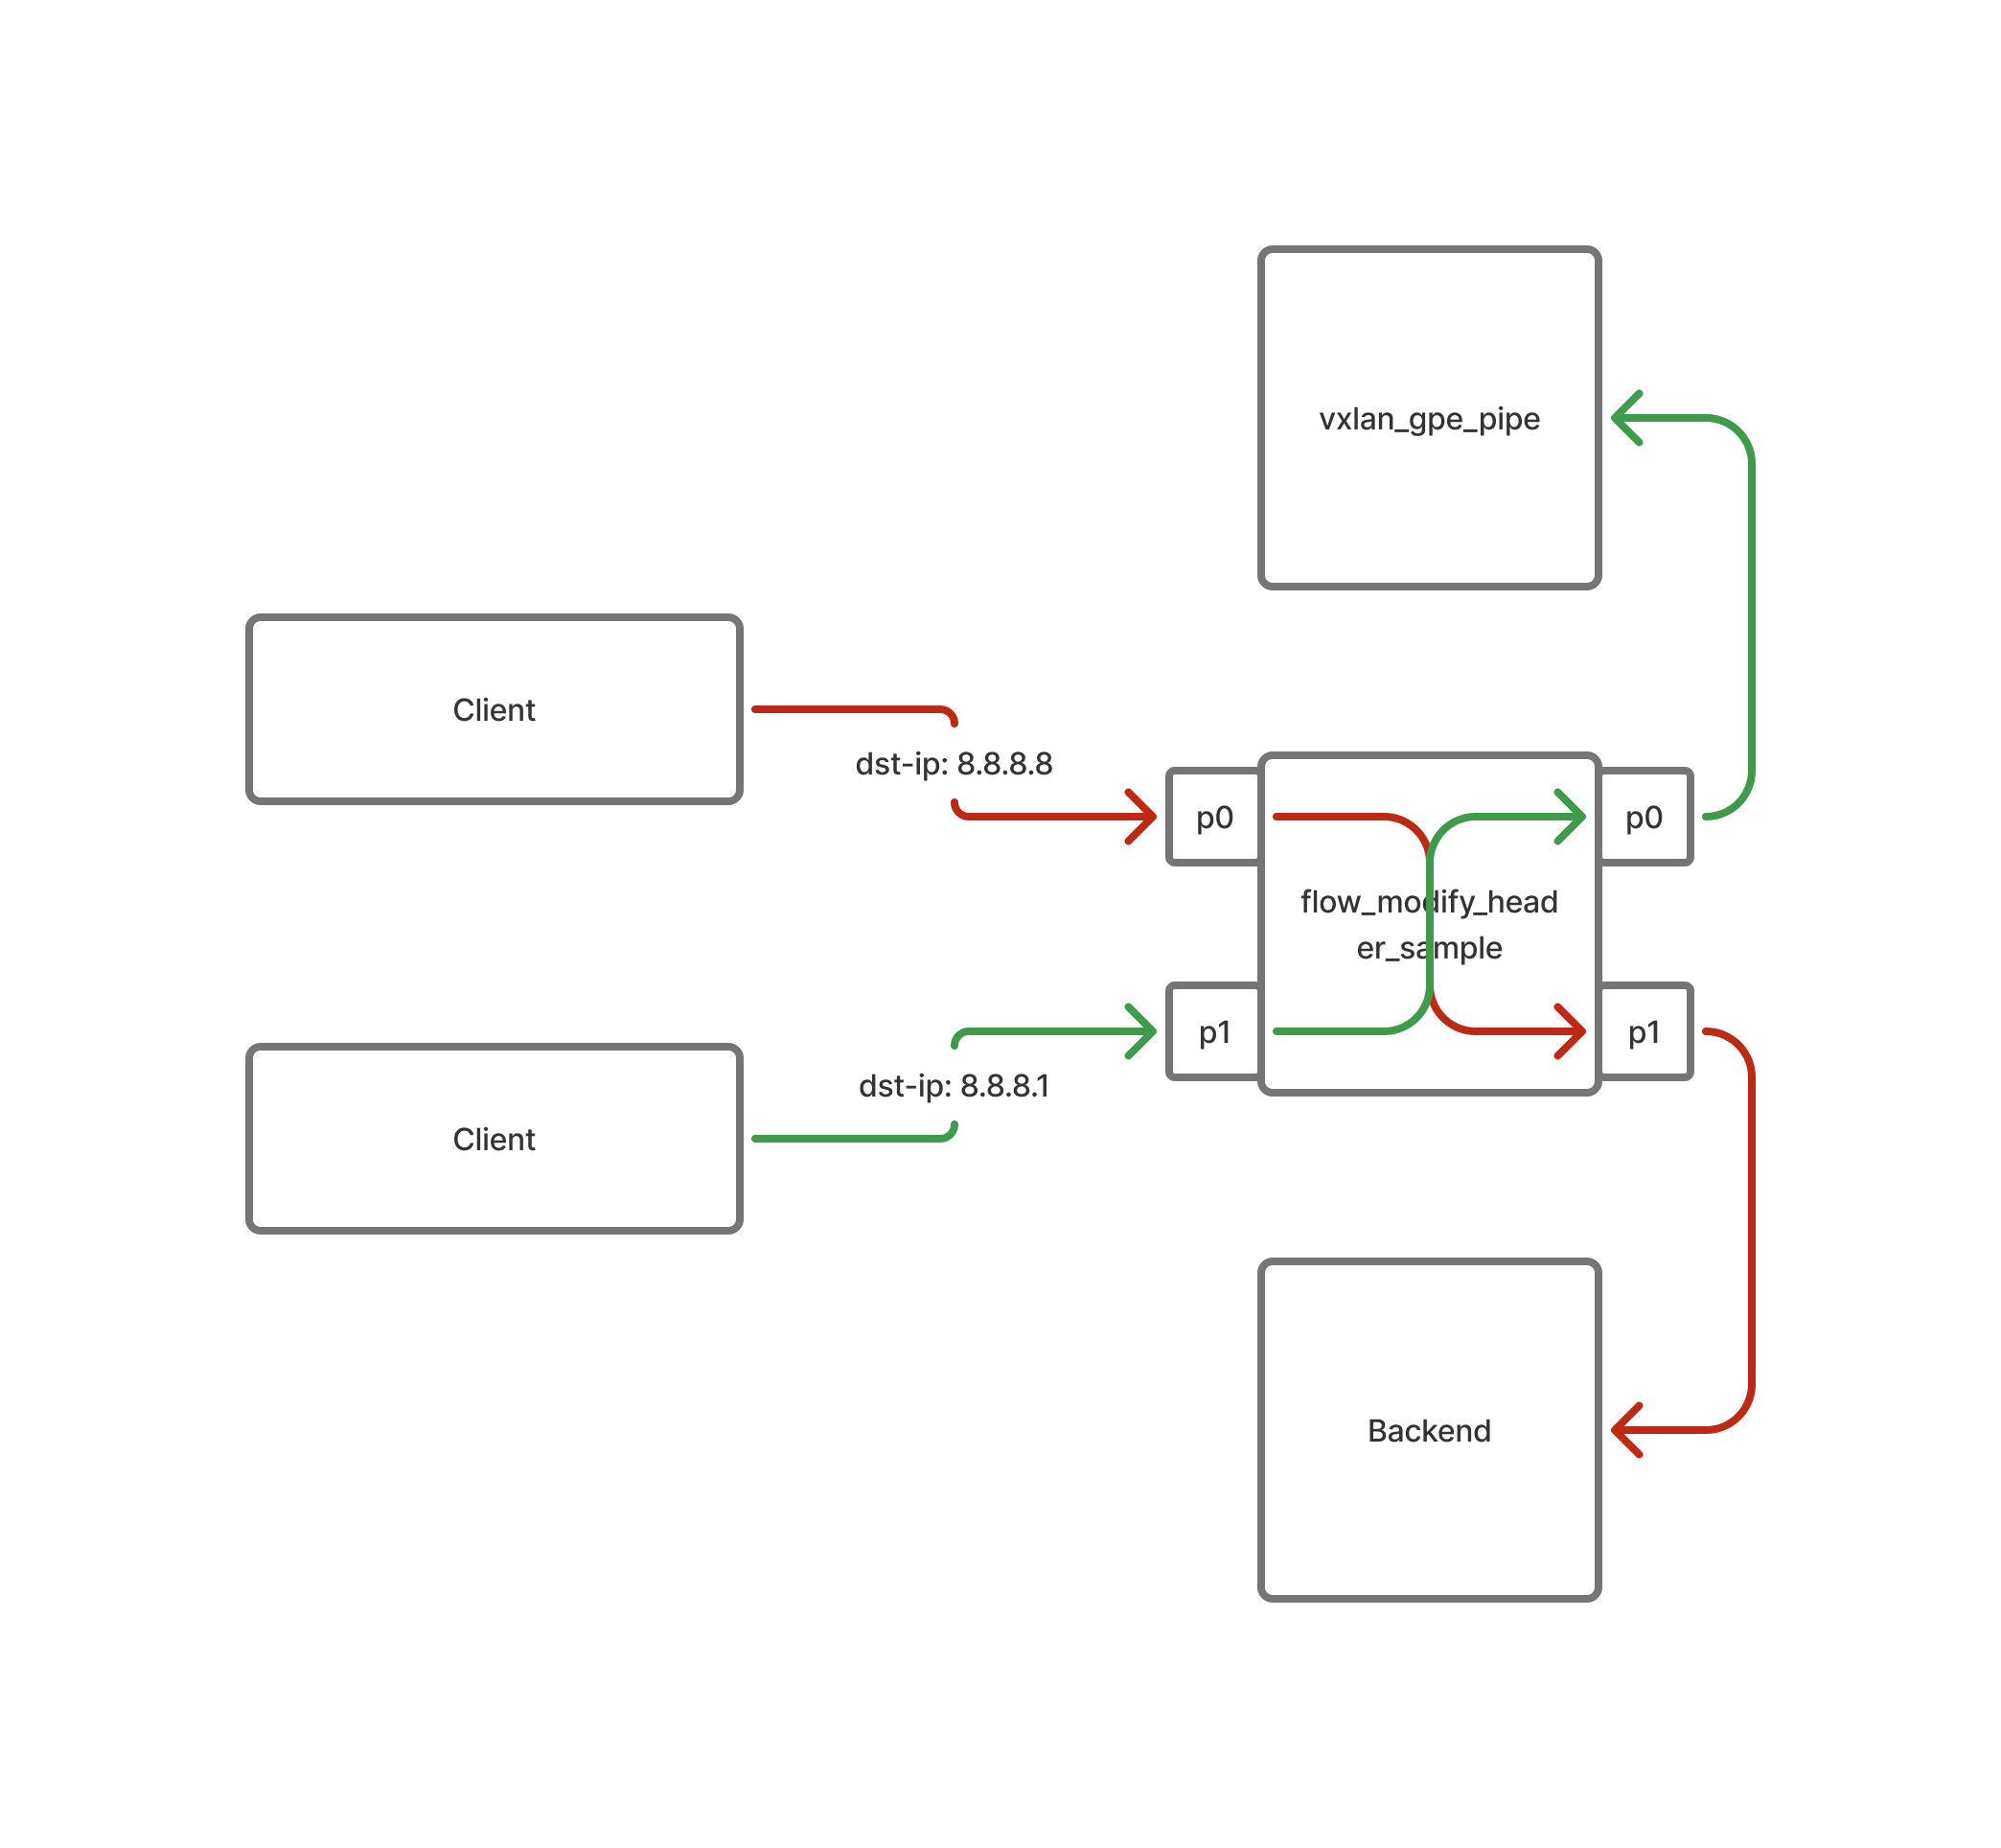
\includegraphics[width=0.8\linewidth]{images/modify_header.png}
    \caption{Flow Modify Header Sample Aufbau}
    \label{fig:enter-label}
\end{figure}
Zu Beginn der Entwicklung wurde auf der Beispielapplikation flow\_modify\_header\_sample.c aufgebaut. Das besagte Beispielprojekt beschreibt eine Anwendung, in der Netzwerkverkehr auf das bestimmte Destination-IP-Feld mit der IP 8.8.8.8 gematcht wird und daraufhin die MAC-Adresse mittels Action geändert wird. Dieser Ansatz ist für die Implementierung eines Load Balancers von großem Interesse. Grund dafür ist, dass ein Netzwerkpaket so manipuliert werden kann, dass es den mit der MAC-Adresse spezifizierten Rechner erreichen kann, dort dann aber eine Modifikation der MAC-Adresse vorgenommen wird, damit das Paket an ein dediziertes Backend weitergeleitet wird. Zusätzlich wurde noch die Beispielapplikation flow\_shared\_counter\_sample.c untersucht. In dieser wird ein Beispiel gegeben, wie von der BlueField erfasste Monitoring-Daten abgerufen werden können, um Informationen über den aktuellen Datenverkehr erhalten zu können. Dies ist, sofern es wirklich Hardwareeinheiten sind, nicht trivial, da es keinen Speicherbereich oder Ähnliches gibt, auf den zugegriffen werden kann, um Daten zu erhalten. DOCA stellt dafür eine Funktion bereit:
\begin{minted}{c}
int doca_flow_shared_resources_query(DOCA_FLOW_SHARED_RESOURCE_COUNTER,
							shared_counter_ids,
							query_results_array,
							nb_ports);
\end{minted}
 Laut der Dokumentation können so mehrere Entries auf den Counter zugreifen bzw. diesen erhöhen. Der gesamte Prozess ist somit vergleichbar mit Thread-Safety bei parallelen Programmen, abgebildet in der DOCA Flow-Semantik mit Flow Entries.

In Abbildung 6.1 ist dargestellt, wie zwei Clients jeweils ein Paket mittels genauer MAC-Adresse an die modify header Applikation schicken. Der rote Pfad beschreibt dabei ein Paket, welches von der ersten Pipe gefangen wird. Daraufhin wird die entsprechende Source MAC-Adresse bearbeitet. Der grüne Pfad beschreibt hingegen ein Paket, welches nicht von der ersten Pipe und deren Entries gefangen wurde. Es wird somit als Miss klassifiziert und in der spezifischen Applikation in eine andere Pipe weitergeleitet. Diese hat im Beispiel nicht für diese Arbeit relevante weitere Operationen in bestimmten Entries definiert. Alle von einem bestimmten Hardwareport der BlueField verarbeiteten Pakete werden an den jeweils anderen Hardwareport weitergeleitet.
\subsection{Grundapplikation}
Im Anschluss an diverse Experimente zum Verständnis von DOCA Flow mithilfe der Beispielapplikationen wurde das Grundgerüst für XenoFlow implementiert. Dazu wurde erstmalig überlegt, wie der Verkehr in verschiedene Teilnetzverkehre aufgeteilt wird, damit dieser dann auf mehrere Backends verteilt werden kann. Zunächst sollte in Anlehnung an die Masterarbeit von Phillip Ungrund ein Algorithmus verwendet werden, der die Source-Adresse im IP Header analysiert und anhand dieser eine Hashsumme errechnet. Diese Hashsumme soll dann überprüft werden, ob sie bereits bekannt ist. Sollte dies der Fall sein, so wird sie an die gleiche Backendadresse weitergeleitet. Wenn nicht, so wird ein Backend zufällig gewählt und ein entsprechender Eintrag in einer Datenstruktur für späteren Netzwerkverkehr angelegt. Dieser Ansatz wurde allerdings im Laufe der weiteren Gespräche in der Gruppe verworfen. Grund dafür ist, dass ein solcher Algorithmus nicht hardwarebeschleunigt laufen könnte. Er müsste von einer der spezialisierten Hardwareeinheiten ausgeführt werden. Diese sind allerdings in ihrer Funktionalität nicht frei programmierbar. Somit müsste jedes unbekannte Datenpaket von einer Hashfunktion analysiert werden, welche auf dem ARM Prozessor ausgeführt wird. Damit würde abermals die Idee der vollständigen Hardwarebeschleunigung verloren gehen und die Performance des Lastverteilers wäre an den Prozessorkern gebunden. Daher wurde zunächst die Untersuchung der tatsächlichen Performance der BlueField-3 Verarbeitung in den Vordergrund gestellt, womit ein wesentlich simplerer, aber deutlich leichter zu implementierender Algorithmus entwickelt wurde. Dazu wird auf der Ebene der Bitfelder die Source-Adresse im IP Header verwendet und mittels des Filter-Matchings überprüft, ob die letzten Bits einer Client-IP einem bestimmten Muster entsprechen.
\begin{figure}
    \centering
    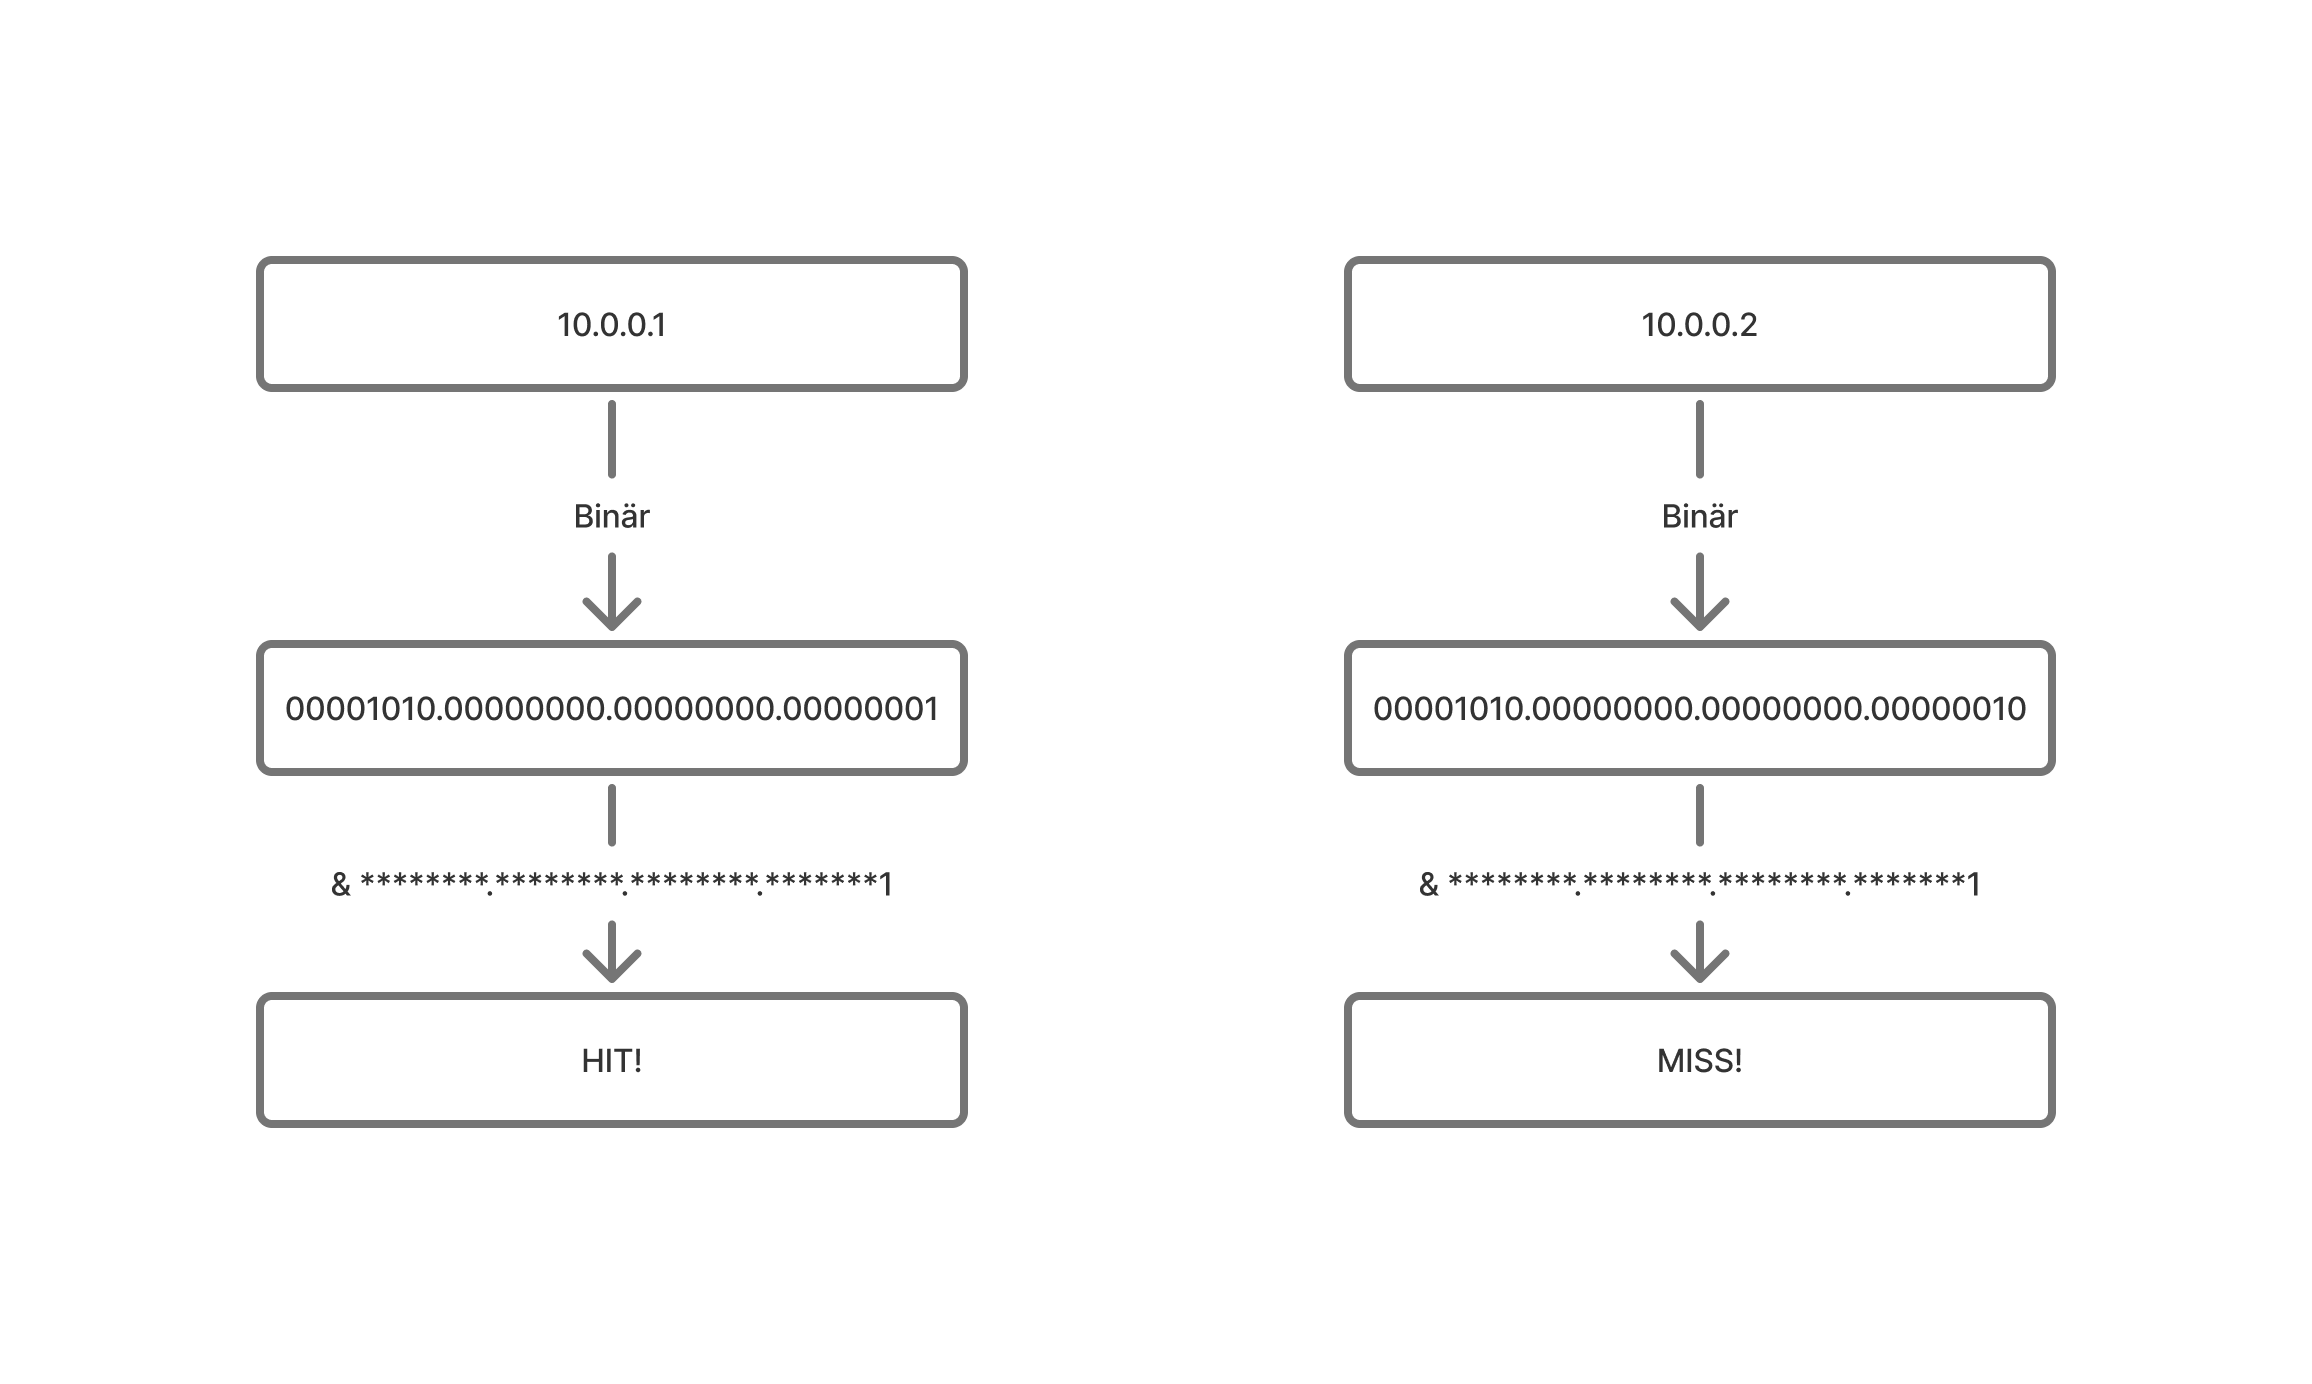
\includegraphics[width=1.1\linewidth]{images/Filter Matching.png}
    \caption{XenoFlow Matching Algorithmus}
    \label{fig:enter-label}
\end{figure}
In Abbildung 6.2 ist ein beispielhafter Aufbau angegeben. Hierbei werden zwei Source-Adressen untersucht. Bei der Adresse 10.0.0.1 ist das letzte Bit der IP gesetzt. Wird also daraufhin der Filter mittels Und-Operator angewendet, so führt diese Adresse zu einem Hit und wird in die entsprechende Pipe eingefügt bzw. von dem entsprechenden Entry verarbeitet. Bei einer IP-Adresse, bei der allerdings das letzte Bit nicht gesetzt ist, wie es bei 10.0.0.2 der Fall ist, wird der Und-Filter das Paket als Miss interpretieren. Der beschriebene Algorithmus beschreibt hier natürlich nur einen Teil, zeigt aber in seinem Aufbau, wie sich anhand leichter Filter zwei Klassen von IP-Adressen erstellen lassen. Genauer in gerade und ungerade IP-Adressen im letzten der 4 Adressfelder. Der große Vorteil dieser Implementierung ist es, dass der Filter vollständig hardwarebeschleunigt arbeiten kann. Es muss somit keinerlei Logik oder ähnliches durchlaufen werden, um die IP-Klassen zu befüllen. Dies sollte sich in den späteren Versuchen deutlich machen.
\subsection{Definition von Backends}
Backends, welche in der Lage sind, Clientanfragen zu bearbeiten und dementsprechend von dem Lastverteiler als valide Endpunkte für eingehenden Verkehr angesehen werden sollen, können in XenoFlow deklarativ definiert werden. Hintergrund dafür ist, dass moderne Systeme wie Kubernetes ebenfalls auf einen deklarativen Konfigurationsstil setzen. Dazu wird die Formatierung \textbf{json} verwendet. 

So können Backends für XenoFlow definiert werden, indem wie folgt JSON-Dateien angelegt werden:
\begin{minted}{json}
{
    "backends": [
        {
            "name": "fips2",
            "mac_address": "A0:88:C2:B5:F4:5A"
        },
        {
            "name": "fips3",
            "mac_address": "E8:EB:D3:9C:71:AC"
        }
    ] 
}
\end{minted}
Dabei spielen die Namen der jeweiligen Backends nur in der Ausgabe von XenoFlow eine Rolle und sind mehr dazu gedacht, bei späteren Weiterentwicklungen von XenoFlow verwendet zu werden. Von größerem Interesse sind die MAC-Adressen, die mit einem jeweiligen Backend assoziiert werden. Diese werden folgend im Lastverteiler verwendet, um eingehende Pakete an diese Adresse weiterzuleiten. Hierbei sei auch erwähnt, dass, ähnlich wie bei DNS-basierten Lastverteilern, im aktuellen Implementierungsstatus nicht sichergestellt ist, ob das jeweilige Backend überhaupt in der Lage ist, Traffic zu verarbeiten. Dies ist allerdings ein Feature, welches sich ebenfalls zu einem späteren Zeitpunkt und unabhängig von dieser Arbeit dazu implementieren lassen würde. Außerdem wäre eine Erweiterung denkbar, die \textbf{yaml} als zusätzliche Markup-Sprache akzeptiert, da YAML wesentlich häufiger in Kontexten wie Kubernetes verwendet wird. Damit wäre XenoFlow ein wenig mehr in line mit modernen Cloudsystemen und deren syntaktischen Entwicklungen.
\newline
Die nun definierten Backends modifizieren die entsprechenden Hardware-Filterregeln. Aufgrund der Natur des gewählten Algorithmus und des binären Zahlensystems ist es im aktuellen Prototypen nur möglich, eine gerade Anzahl von Backends zu deklarieren. Aber auch diese Beschränkung lässt sich durch die Wahl von anderen Netzwerkverkehrsklassifizierungsalgorithmen umgehen. Würde eine Erweiterung hinsichtlich der Health Checks sowie anderer Funktionalitäten wie Logging erfolgen, so ist es dringend angeraten, die allgemeine Architektur der Backendwahl zu modifizieren. Im Rahmen dieser Arbeit wurde die Architektur allerdings bewusst einfach gehalten, um die tatsächliche Leistung der BlueField zu beurteilen und nicht die der entsprechenden Architektur.
\subsection{Open vSwitch}
\begin{figure}
    \centering
    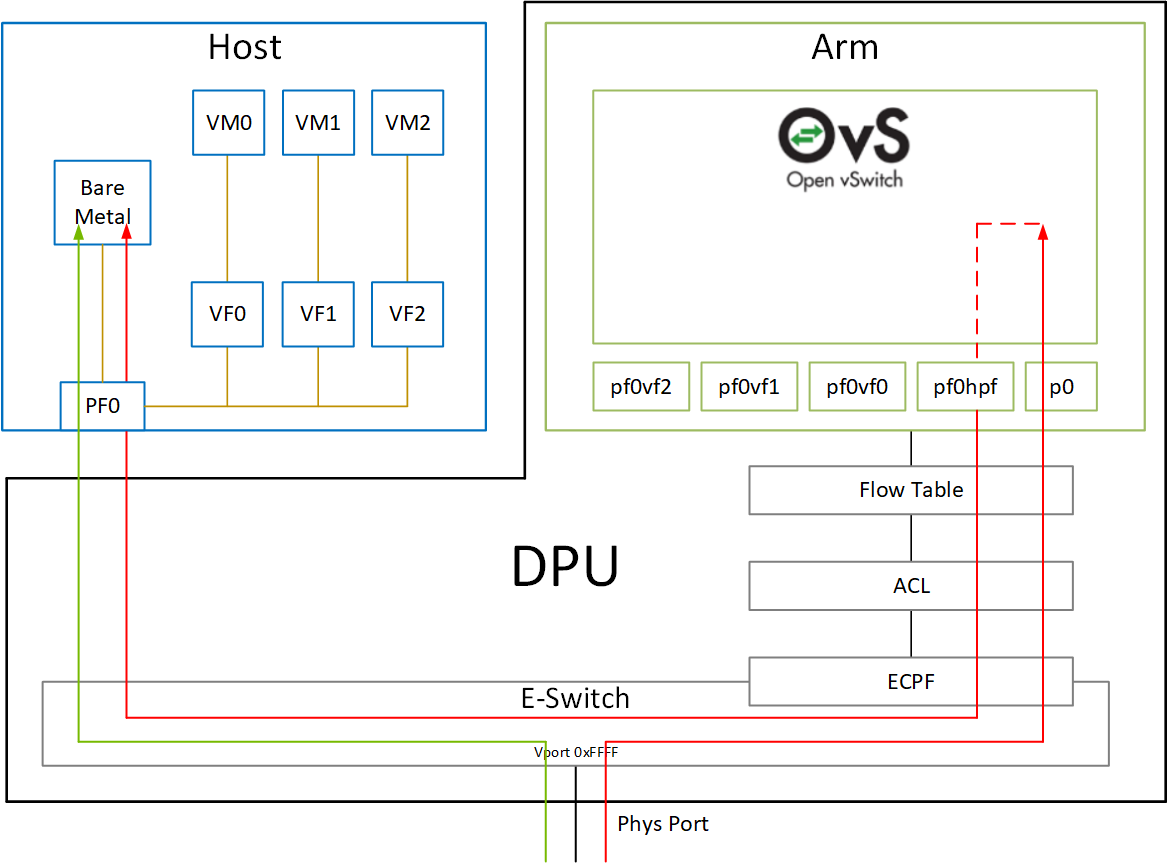
\includegraphics[width=0.85\linewidth]{images/kernel_representors_model.png}
    \caption{Open vSwitch auf der BlueField-3}
    \label{fig:enter-label}
\end{figure}
Die Bluefield verwendet, wie in den vorherigen Kapiteln beschrieben, virtuelle Netzwerkinterfaces, um zwischen dem Host und den ARM-Kernen zu kommunizieren, aber auch, um den Verkehr zwischen den Hardwareport zu steuern. Dazu verwendet NVidia Open vSwitch. Open vSwitch ist eine Applikation, um die Funktionalität eines Switches, der Multilayer arbeiten kann, per Software in Linux abzubilden. Das Projekt wird von der Linux Foundation entwickelt und ist komplett quelloffen unter der Apache-Lizenz 2.0 veröffentlicht. Laut NVidia werden Switch-Regeln, die in Open vSwitch angelegt werden, mittels der ASAP²-Technologie auf die Hardwarebeschleuniger ausgelagert. Dazu ist in Abbildung 6.3 ein Datenpfad von zwei unterschiedlichen Paketen abgezeichnet. Der grüne Pfad zeigt ein Paket, welches direkt vom Switch an den Host hochgereicht wird und dort unter dem Interface PF0 abgeholt werden kann. Das Paket des roten Pfades hingegen durchläuft zunächst den ARM-Kern mit den entsprechenden Interfaces. Unsere Lastverteilung allerdings soll keinen der beiden angegebenen Pfade durchlaufen, sondern lediglich auf den Hardwarebeschleunigern ausgeführt werden. Somit muss allerdings auch deklariert werden, dass eingehender Traffic direkt wieder aus dem entsprechenden anderen Hardwareport ausgegeben wird. Dies ist dank der Erweiterung von OVS von NVidia möglich. Diese Erweiterung trägt den Namen NVIDIA's DOCA-OVS. Im Speziellen soll DOCA-OVS API-Aufrufe ergänzen, die ermöglichen, dass die Hardware entsprechend mit den definierten Regeln arbeiten kann.
\section{Quellcode}
Im folgenden Abschnitt wird ein genauer Überblick über den XenoFlow Lastverteiler gegeben. Es werden die verschiedenen C-Strukturen und Funktionen, die intrinsisch von NVidia bereitgestellt werden, vorgestellt. 
\subsection{main()}
Zu jeder Flow-Applikation gehören nicht nur die entsprechenden Datenstrukturen zur Definition von Pipes und Entries, sondern es müssen auch Konfigurationen allgemeinerer Natur getroffen werden. Diese werden allgemein in einer \_main.c zusammengefasst. In dieser Quellcode-Datei liegt außerdem die eigentliche main Funktion, die zu Beginn eines jeden C Programms ausgeführt wird.
\begin{minted}{c}
int main(int argc, char **argv)
{
	doca_error_t result;
	struct doca_log_backend *sdk_log;
	int exit_status = EXIT_FAILURE;
	struct application_dpdk_config dpdk_config = {
		.port_config.nb_ports = 2,
		.port_config.nb_queues = 4,
		.port_config.nb_hairpin_q = 2,
	};
\end{minted}
Zunächst werden hier einige Datenstrukturen deklariert. Interessant sind hierbei die\newline\texttt{doca\_log\_backend} und \texttt{application\_dpdk\_config} Strukturen.

Das Logbackend wird verwendet, um festzulegen, wie und welches Loglevel erfasst werden soll.
Hierzu wird mit den intrinsischen Funktionsaufrufen
\begin{minted}{c}
result = doca_log_backend_create_standard();
if (result != DOCA_SUCCESS)
    goto sample_exit;
result = doca_log_backend_create_with_file_sdk(stderr, &sdk_log);
if (result != DOCA_SUCCESS)
    goto sample_exit;
result = doca_log_backend_set_sdk_level(sdk_log, DOCA_LOG_LEVEL_WARNING);
if (result != DOCA_SUCCESS)
    goto sample_exit;
\end{minted}
die entsprechende Struktur initialisiert und \texttt{stderr} als Output-Zeiger übergeben. Hier könnten theoretisch auch andere Ziele für die entsprechenden Lognachrichten festgelegt werden. Außerdem wird das minimale Loglevel festgelegt. Lognachrichten, die unter diesem Loglevel liegen, werden nicht angezeigt. Es haben sich hierbei folgende Loglevel entwickelt, die auch in DOCA verwendet werden können:
\begin{itemize}
    \item DEBUG - Sehr verbose und ausführliche Informationen zum auffinden von Fehlern im Betrieb
    \item INFO - Allgemeine Informationen über den Programmstatus
    \item WARNING - Warnungen über eventuell aufkommende Fehler
    \item ERROR - Direkte Fehlermeldungen
\end{itemize}
Eine klassische Lognachricht des Levels INFO sieht wie folgt aus:
\begin{minted}{c}
DOCA_LOG_INFO("Starting the load balancer");
\end{minted}
Als nächstes wird DPDK initialisiert. Dazu wird abermals mittels einer DOCA intrinsischen Funktion die zuvor erstellte Datenstruktur übergeben und außerdem wird der Name, der folgend als ID für die laufende DOCA Applikation verwendet wird, festgelegt:
\begin{minted}{c}
doca_argp_init("doca_flow_lb", NULL);

doca_argp_set_dpdk_program(dpdk_init);

doca_argp_start(argc, argv);
\end{minted}
Mittels des letzten Funktionsaufrufs werden die Parameter der Konsole mit an DOCA übergeben. Dies ist vor allem dazu gebräuchlich, um zu deklarieren, über welches PCI Interface mit der BlueField kommuniziert werden soll, da es möglich ist, mehrere BlueFields in einem Host zu verbauen.
Zuletzt wird nun unsere eigentliche Applikation ausgeführt:
\begin{minted}{c}
xeno_flow(dpdk_config.port_config.nb_queues);
\end{minted}
\subsection{xeno\_flow()}
Als erstes findet die Deklaration sämtliche Datenstrukturen deklariert, die im Folgenden von XenoFlow gebraucht werden:
\begin{minted}{c}
int nb_ports = 1;
struct flow_resources resource = {1};
uint32_t nr_shared_resources[SHARED_RESOURCE_NUM_VALUES] = {0};
struct doca_flow_port *ports[2];
struct doca_dev *dev_arr[nb_ports];
struct doca_flow_pipe *udp_pipe;
int port_id = 0;
uint32_t shared_counter_ids[] = {0, 1};
struct doca_flow_resource_query query_results_array[nb_ports];
struct doca_flow_shared_resource_cfg cfg = {.domain = DOCA_FLOW_PIPE_DOMAIN_DEFAULT};
struct entries_status status;
int num_of_entries = 4;
doca_error_t result;
nr_shared_resources[DOCA_FLOW_SHARED_RESOURCE_COUNTER] = 2;
XenoFlowConfig *config = load_config();
\end{minted}
Hier wird definiert, wie viele Ports von XenoFlow verwendet werden sollen (allerdings nur, wie viele später mit Pipes genutzt werden; es kann auf mehr Ports weitergeleitet werden) und es werden die Strukturen für die späteren Pipedefinitionen festgelegt. Außerdem wird in der letzten Zeile die Konfiguration aus der \texttt{backends.json} geladen. Diese kann dann später vom Lastverteilungsalgorithmus verwendet werden. In DOCA Flow wird ein sehr expliziter Programmierstil gefordert. Es muss stets genau angegeben werden, wie viele Elemente von Strukturen an DOCA übergeben werden. So muss beispielsweise die Anzahl an Entries in den Pipes klar angegeben sein.
\newline
Nun können die eigentlichen Konfigurationsfunktionen aufgerufen werden. Es sei kurz erwähnt, dass die Flow-Beispielapplikationen meist das Errorhandling mittels eines \texttt{if} realisieren. Da dies zu einem enorm langen und teils unleserlichen Quelltext führt, wurde die Funktion \texttt{doca\_try} implementiert, die im Wesentlichen nur den \texttt{return} des Funktionsaufrufs überprüft. Ist dieser != DOCA\_SUCCESS, so wird eine Fehlermeldung ausgegeben. Damit konnte der Quellcode um ca. 100 Zeilen verkürzt werden.
\begin{minted}{c}
DOCA_LOG_INFO("Number of backends: %d", config->numBackends);

doca_try(
    init_doca_flow(
        nb_queues, 
        "vnf,hws", 
        &resource, 
        nr_shared_resources
    ), "Failed to init DOCA Flow", nb_ports, ports
);

doca_try(
    init_doca_flow_ports(
        2, 
        ports, 
        true, 
        dev_arr
    ), "Failed to init DOCA ports", nb_ports, ports
);

doca_try(
    doca_flow_shared_resource_set_cfg(
        DOCA_FLOW_SHARED_RESOURCE_COUNTER, 
        0, 
        &cfg
    ), "Failed to configure shared counter to port", nb_ports, ports
);



doca_try(
    doca_flow_shared_resources_bind(
        DOCA_FLOW_SHARED_RESOURCE_COUNTER, 
        &shared_counter_ids[0], 
        1, 
        ports[0]
    ), "Failed to bind shared counter to pipe", nb_ports, ports
);

\end{minted}
Mittels \texttt{init\_doca\_flow()} wird DOCA Flow initialisiert. Somit wird sichergestellt, dass die API, die mit den Hardwareeinheiten kommuniziert, verfügbar ist und auf kommende Eingaben wartet. Selbiges gilt für \texttt{init\_doca\_flow\_ports()}. Hier werden die entsprechenden beiden Hardwareports an der Netzwerkkarte angewiesen, dass nun Traffic erwartet werden kann, der mittels Steering-Regeln aus DOCA Flow kontrolliert wird. Anschließend werden mittels \texttt{doca\_flow\_shared\_resources\_bind()} die Counter-Ressourcen gebunden. Diese werden im späteren Programmablauf verwendet, um einen Livestatus über die verteilte Last zu erhalten. Diese Ressource muss abermals intrinsisch an DOCA Flow übergeben werden, damit das entsprechende Hardwarebackend angesprochen werden kann.
\begin{minted}{c} 
doca_try(
    create_root_pipe(
        ports[0], 
        0, 
        DOCA_FLOW_L4_TYPE_EXT_UDP, 
        &udp_pipe
    ), "Failed to create pipe", nb_ports, ports
);

doca_try(
    add_shared_counter_pipe_entry(
        udp_pipe, 
        DOCA_FLOW_L4_TYPE_EXT_UDP, 
        shared_counter_ids[0], 
        &status
    ), "Failed to add entry", nb_ports, ports
);

doca_try(
    doca_flow_entries_process(
        ports[0], 
        0, 
        DEFAULT_TIMEOUT_US, 
        num_of_entries
    ), "Failed to process entries", nb_ports, ports
);
\end{minted}
Nun werden die beiden entscheidenden Funktionen \texttt{create\_root\_pipe()} und \newline\texttt{add\_shared\_counter\_pipe\_entry()} aufgerufen. Diese beinhalten die entsprechende Lastverteilungslogik. Zuletzt wird DOCA Flow angewiesen, die angelegten Entries zu verarbeiten. In diesem Schritt findet die eigentliche Hardwareauslagerung statt. Die Funktion dazu lautet \texttt{doca\_flow\_entries\_process()}.
\subsection{Pipe und Entry Erstellung}
\textit{Die folgenden Quellcodeabschnitte wurden aufgrund der besseren Lesbarkeit leicht gekürzt.}
Im folgenden Code ist zunächst die Erstellung einer Pipe, die zunächst sämtlichen Netzwerkverkehr abfängt:
\begin{minted}{c}
static doca_error_t create_root_pipe(
    struct doca_flow_port *port,
    int port_id,
    enum doca_flow_l4_type_ext out_l4_type,
    struct doca_flow_pipe **pipe
) {
    struct doca_flow_match match;
    struct doca_flow_match match_mask;
    struct doca_flow_monitor monitor;
    struct doca_flow_actions actions0, *actions_arr[2];
    struct doca_flow_fwd fwd, fwd_miss;
    struct doca_flow_pipe_cfg *pipe_cfg;
    
    match.outer.l3_type = DOCA_FLOW_L3_TYPE_IP4;
    match.outer.ip4.src_ip = BE_IPV4_ADDR(255, 255, 255, 255);
    match_mask.outer.ip4.src_ip = BE_IPV4_ADDR(0, 0, 0, 1);
    DOCA_LOG_INFO("%d", match_mask.outer.ip4.src_ip);
    
    SET_MAC_ADDR(
        actions0.outer.eth.dst_mac, 
        0xff, 0xff, 0xff, 0xff, 0xff, 0xff
    );
    SET_MAC_ADDR(
        actions0.outer.eth.src_mac, 
        0xff, 0xff, 0xff, 0xff, 0xff, 0xff
    );
    actions_arr[0] = &actions0;
    monitor.counter_type = DOCA_FLOW_RESOURCE_TYPE_SHARED;
    monitor.shared_counter.shared_counter_id = 0xffffffff;
    
    doca_flow_pipe_cfg_create(&pipe_cfg, port);
    set_flow_pipe_cfg(
        pipe_cfg, 
        "SHARED_COUNTER_PIPE", 
        DOCA_FLOW_PIPE_BASIC, 
        true
    );
    doca_flow_pipe_cfg_set_match(pipe_cfg, &match, &match_mask);
    doca_flow_pipe_cfg_set_actions(pipe_cfg, actions_arr, NULL, NULL, 1);
    doca_flow_pipe_cfg_set_monitor(pipe_cfg, &monitor);
    
    fwd.type = DOCA_FLOW_FWD_PORT;
    fwd.port_id = 1;
    fwd_miss.type = DOCA_FLOW_FWD_DROP;
    
    doca_flow_pipe_create(pipe_cfg, &fwd, &fwd_miss, pipe);
}
\end{minted}
Wie schon in Kapitel 3 dem Aufbau einer Pipe zu entnehmen ist, besteht eine Pipe grundsätzlich aus den Elementen \textbf{Match}, \textbf{Monitor}, \textbf{Action} und \textbf{Forward}. Diese werden mittels entsprechender DOCA Flow Structs deklariert und mit den entsprechenden Werten gefüllt. Hierzu sei erwähnt, dass damit alle Bits für das Matching oder eine spätere Action als aktiv geschaltet sein müssen. Sollen sie also im späteren Programmablauf gelesen oder modifiziert werden können, müssen die entsprechenden Bits in der Pipe-Deklaration als 1 gesetzt werden. Dazu sind z.B. die Counter-ID auf \texttt{0xffffffff} oder die src\_mac auf \texttt{0xff, 0xff, 0xff, 0xff, 0xff, 0xff}. Mit der Erstellung der Pipe sollten die entsprechenden Bitfelder auf der Hardware der BlueField-3 aktiviert sein. Außerdem muss, da wir einen impliziten Match forcieren wollen, eine zweite Filtermaske gesetzt werden, die bei Aufruf der intrinsischen Funktion \texttt{doca\_flow\_pipe\_cfg\_set\_match()} mit übergeben wird. Außerdem müssen bereits die \texttt{doca\_flow\_actions} angegeben werden, die in den einzelnen Entries zur Anwendung kommen. Dabei wird nicht spezifiziert, was genau modifiziert werden soll, sondern nur, welche Bitfelder zur Modifikation freigegeben sind.

Zuletzt wird mittels der Funktion \texttt{doca\_flow\_pipe\_create()} die entsprechende Pipe final angelegt. Ist dieser Funktionsaufruf ohne Fehlermeldung und erfolgreich, so ist die Hardwaresteering-Regel aktiv und der Traffic wird nun gemäß den angelegten Regeln verarbeitet.
\newline Da mit der Pipe noch nicht die spezielle Lastverteilung eingebaut ist, sondern lediglich definiert wurde, welche Bitfelder verarbeitet werden sollen und welcher Traffic überhaupt abgegriffen werden soll, ist im folgenden Quelltext die Erstellung der beiden speziellen Entries angegeben:
\begin{minted}{c}
static doca_error_t add_shared_counter_pipe_entry(
    struct doca_flow_pipe *pipe,
    enum doca_flow_l4_type_ext out_l4_type,
    uint32_t shared_counter_id,
    struct entries_status *status
) {
    /**
        ...
    **/
    
    monitor.shared_counter.shared_counter_id = shared_counter_id;
    
    match.outer.ip4.src_ip = BE_IPV4_ADDR(0, 0, 0, 1);	
    actions.action_idx = 0;
    SET_MAC_ADDR(
        actions.outer.eth.dst_mac, 
        0xe8, 0xeb, 0xd3, 0x9c, 0x71, 0xac
    );
    SET_MAC_ADDR(
        actions.outer.eth.src_mac, 
        0xc4, 0x70, 0xbd, 0xa0, 0x56, 0xbd
    );
    doca_flow_pipe_add_entry(
        0, 
        pipe, 
        &match, 
        &actions, 
        &monitor, 
        NULL, 
        0, 
        status, 
        &entry_mac
    );
    /**
        ...
    **/
    return DOCA_SUCCESS;
}
\end{minted}
In diesem letzten, aber auch wichtigsten Codeabschnitt findet der tatsächliche MAC-Adressen-Rewrite statt. Zunächst wird nun der explizite Filterteil auf der Ebene eines einzelnen Entry gesetzt. Dazu erhält die Match-Datenstruktur ein IP-Bitfeld, bei dem nur das letzte Bit gesetzt ist. Das heißt, dieses Entry fängt alle Pakete ab, deren Source-IP-Adresse auf dem letzten Bit eine 1 gesetzt hat. Daraufhin muss die Action ID definiert werden. Diese Action ID wird vor allem zum späteren Logging verwendet, um zu überprüfen, wie viele Pakete von dieser Action verarbeitet wurden. Anschließend sind die entsprechenden MAC-Adressen in der \texttt{actions.outer.eth.dst\_mac} und der \texttt{actions.outer.src\_mac} angegeben.
Mittels \texttt{doca\_flow\_pipe\_add\_entry()} kann nun der entsprechenden Pipe das Entry zugeordnet werden. Das im Code gezeigte Entry ist lediglich eines für ein entsprechendes Backend, dessen MAC-Adresse in der dst\_mac angegeben wird. Sollen nun mehr Backends hinzugefügt werden, benötigt es eine abermalige Ausführung. 
\subsection{Logging und Datenerfassung}
Der XenoFlow Lastverteiler hat eine Echtzeit-Datenerfassung mit implementiert. Dazu wird in einem periodischen Intervall ein 
\begin{minted}{c}
doca_flow_shared_resources_query(
    DOCA_FLOW_SHARED_RESOURCE_COUNTER,
    shared_counter_ids,
    query_results_array,
    nb_ports
);
\end{minted}
Aufruf gemacht. Dessen Ergebnis ist eine Datenstruktur, die einfach ausgelesen werden kann, um die entsprechenden Werte zur Laufzeit auf der Kommandozeile ausgeben zu können.

\subsection{Bemerkung}
Alle Funktionalitäten sind aus dem von NVidia bereitgestellten Headerfile\texttt{ doca\_flow.h} entnommen worden. Die tatsächlichen Implementationen sind \textbf{nicht} quelloffen. Es ist nicht ersichtlich, welche Algorithmen zur Anwendung kamen. Die gegebene Headerdatei ist zwar kommentiert, es wäre allerdings deutlich einfacher, das Projekt quelloffen zu halten, sodass ein genauerer Einblick in die interne Funktionsweise ermöglicht wird. Die Libraries werden als .so-Dateien bereitgestellt.
    
    \acresetall % reset acronym counter
    %
% chapter5.tex
%

\chapter{Messungen und Experimente}
\label{cha:experiments}

\section{...}
Justo eget magna fermentum iaculis eu. Tristique et egestas quis ipsum suspendisse ultrices gravida dictum. Luctus accumsan tortor posuere ac ut consequat semper viverra. Duis ut diam quam nulla porttitor massa id neque aliquam. Tellus mauris a diam maecenas sed enim. Et leo duis ut diam quam nulla porttitor massa. Id aliquet lectus proin nibh nisl condimentum id venenatis a. Eros in cursus turpis massa tincidunt. Sed pulvinar proin gravida hendrerit lectus. Gravida arcu ac tortor dignissim. Est ullamcorper eget nulla facilisi etiam. Netus et malesuada fames ac.


    \acresetall % reset acronym counter
    %
% chapter6.tex
%

\chapter{Zusammenfassung \& Ausblick}
Lorem ipsum dolor sit amet, consectetur adipiscing elit, sed do eiusmod tempor incididunt ut labore et dolore magna aliqua. Erat nam at lectus urna. Vitae purus faucibus ornare suspendisse sed nisi lacus. Turpis egestas integer eget aliquet nibh praesent tristique magna. Et netus et malesuada fames ac turpis egestas. Nunc vel risus commodo viverra maecenas accumsan lacus. Nisi scelerisque eu ultrices vitae auctor eu augue. Odio morbi quis commodo odio aenean sed adipiscing. Ultricies lacus sed turpis tincidunt id aliquet. Sit amet mattis vulputate enim nulla aliquet porttitor lacus luctus. Tellus rutrum tellus pellentesque eu tincidunt tortor.

    
    %
% outro.tex
%

\addtocontents{toc}{\protect\newpage}
% start the appendix (changes section numbering, and others)
\appendix
% use different page style
\pagestyle{appendixstyle}
%reset acronym counter
% \acresetall % really? (by stefan)

%
% list of figures
%

\listoffigures
%\cleardoublepage

%
% list of tables
%

\listoftables
%\cleardoublepage

%
% list of algorithms
%

\listofalgorithms
%\cleardoublepage

\clearpage

%
% list of abbreviations
%

\iflanguage{ngerman}
{
\chapter{Abkürzungsverzeichnis}
}{
\chapter{Abbreviations}
}
\begin{acronym}[TDMA]
 \acro{CDMA}{Code Division Multiple Access}
 \acro{GSM}{Global System for Mobile communication}
 \acro{NA}[\ensuremath{N_{\mathrm A}}]{Number of Avogadro\acroextra{ (see \S\ref{Chem})}}
 \acro{NAD+}[NAD\textsuperscript{+}]{Nicotinamide Adenine Dinucleotide}
 \acro{NUA}{Not Used Acronym}
 \acro{TDMA}{Time Division Multiple Access}
 \acro{UA}{Used Acronym}
 \acro{lox}[\ensuremath{LOX}]{Liquid Oxygen}%
 \acro{lh2}[\ensuremath{LH_2}]{Liquid Hydrogen}%
\end{acronym}

\chapter{Source Files}
The source files and the corresponding repository can be accessed by contacting the second supervisor: Max Schrötter.

%
% bibliography
%

\printbibliography

\printindex 
 % Appendix etc.

\end{document}
